%%%%%%%%%%%%%%%%%%%%%%%%%%%%%%%%%%%%%%%%%%%%%%%%%%%%%%%%%%%%%%%%%%%%%%%%
\chapter{Method}\label{chap:Method}
%%%%%%%%%%%%%%%%%%%%%%%%%%%%%%%%%%%%%%%%%%%%%%%%%%%%%%%%%%%%%%%%%%%%%%%%

This chapter explains our principle approach on how to extract ridge
features from uncertain scalar fields. In the usual case, ridges do not
lie directly on the nodes of a cell, but inbetween. Therefore it is
insufficient to only look at single nodes of every member of the set of
possibly correlated scalar fields to decide on the presence of a ridge.
Thus, in the $3$-dimensional case, the actual node at the location we
examine is the bottom left node of a cell of 8 nodes (see red node in
Figure~\ref{fig:3DNH}). This follows an implementation detail, as our
scalar fields are traversed from bottom left to top right. Sampling
these 8 nodes with a Monte-Carlo method would only give us Gaussian
distributed values over the range of values at these locations, but no
information about their change along the dimensions outside the cell.\\

\begin{figure}[t]
    \centering
    \begin{subfigure}{0.49\textwidth}
        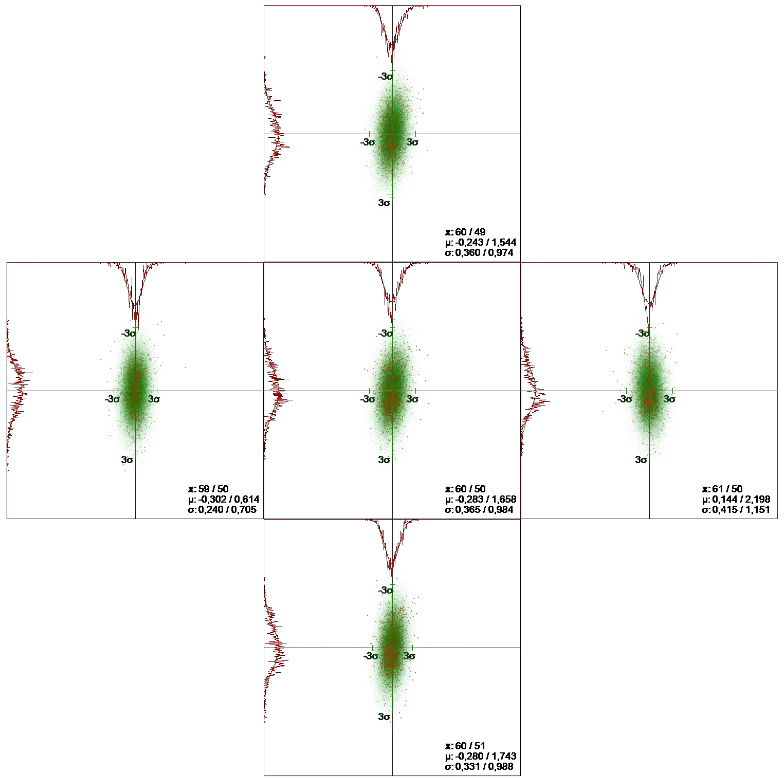
\includegraphics[width=\textwidth]{Images/uncvelocity.png}
        \caption{Uncertain velocity}
        \label{fig:uncvel}
    \end{subfigure}
    \begin{subfigure}{0.49\textwidth}
        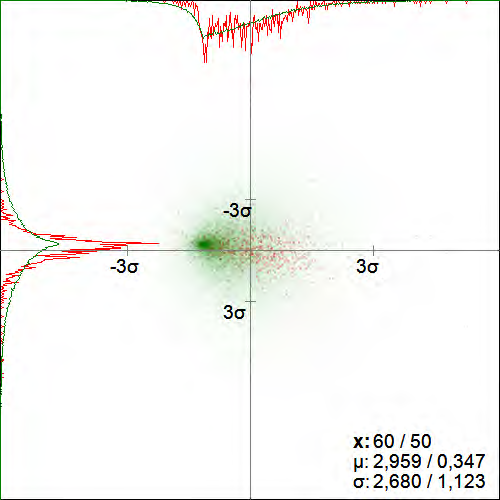
\includegraphics[width=\textwidth]{Images/uncacceleration.png}
        \caption{Uncertain acceleration}
        \label{fig:uncacc}
    \end{subfigure}
    \caption{\subref{fig:uncvel} Distribution of velocity vectors of a
    neighborhood in a 2-dimensional domain. Marginal density
    distributions of the original vectors, shown as red dots, are
    denoted with the red curves. Due to the relatively low member size
    of 1024 vectors, the curves are non-smooth. The green dots and lines
    are the uncorrelated Gaussian reconstruction of the distributions
    calculated from the measured vectors with 100,000 samples. The
    curves show that a Gaussian distribution is indeed a suitable
    choice and the Monte-Carlo reconstruction delivers a correct result.
    \subref{fig:uncacc} Measured acceleration and density distribution
    as red points and curves. Acceleration from uncorrelated Gaussian
    samples and density distribution as green points and curves. The lines
    do not coincide anymore, indicating that the derivatives are not
    following the distribution of their vectors. Images from Otto and
    Theisel~\cite{Vortex}.}
    \label{fig:Theisel}
\end{figure}
\indent Otto and Theisel~\cite{Vortex} tested in their work to derive a
velocity vector $v$ in a two dimensional uncertain vector field by
sampling the vector and its four neighboring vectors individually from
their distributions. They then estimated the Jacobian $J$ with central
differences on the neighboring samples and multiplied it with the
velocity vector, to get the acceleration vector $a = J v$
(Figure~\ref{fig:Theisel}). The resulting vectors did not match the
distribution of the original acceleration vectors anymore. This is a
crucial problem for the extraction of features which are heavily
dependent on correct derivatives. Instead of sampling each vector
individually, they solved this issue by sampling the whole neighborhood
of the vector to keep track of its change along the dimensions.
Therefore we also inspect the 24 nodes adjacent to the 8 nodes of the
cell, to be able to calculate the gradient via central differences. As
Theisel \etal\ were searching for vortex core lines in uncertain vector
fields, they only needed to derive their field once, to be able to
decide on the presence of a core line based on the eigenspace. As we
base our detections on eigenvalues and eigenvectors as well, we need to
derive our uncertain scalar field twice. We therefore also add the
adjacent nodes of the 24 supporting nodes to our considered
neighborhood. This leads to 80 nodes making up the cell we want to draw
samples from (see Figure~\ref{fig:NH}). With this we can create the
uncertain scalar field from Section~\ref{sec:USF}. It is important to
remember that we cannot compute ridge lines and surfaces directly on the
uncertain scalar field, but on samples from it. Thus we sample the field
multiple times and the result is a probability for the existence of the
desired ridge feature in the cell. The next section will explain the
sampling of the distributions in detail.

%%%%%%%%%%%%%%%%%%%%%%%%%%%%%%%%%%%%%%%%%%%%%%%%%%%%%%%%%%%%%%%%%%%%%%%%
\section{Multivariate Gaussian Sampling}\label{sec:MGS}
%%%%%%%%%%%%%%%%%%%%%%%%%%%%%%%%%%%%%%%%%%%%%%%%%%%%%%%%%%%%%%%%%%%%%%%%

Our uncertain scalar field $S_{\mathcal{N}}$ at point
$x=(x_1,\dots,x_n)$ consists of a multivariate Gaussian distribution,
made up from the mean vector $\mu_x$ and the covariance matrix
$\Sigma_x$. The mean vector portrays the average values of the
neighborhood of $x$, while the covariance matrix contains the variances
of each value to each other around this mean. Unfortunately, we cannot
compute ridge criteria from these objects directly. Monte-Carlo methods
offer a way to draw samples from multivariate normal distributions. The
basis of multivariate Gaussian sampling is the affine transformation
property of normal distributed vectors that states that any linear
transformation of a normal vector is again normal:

\begin{equation}
    X \sim \mathcal{N}(\mu,\Sigma) \Rightarrow AX \sim \mathcal{N}(A\mu, A\Sigma A)
\end{equation}

\noindent for any dimensionality $d$ of vector $X$ and $d \times d$
matrix $\Sigma$ and any $k \times d$ matrix $A$. By this property we
know that if we have a standard normal distributed vector $N \sim
\mathcal{N}(0,I)$ with $I$ being an $d \times d$ identity matrix, then
$X = AN + \mu$ is from the distribution $X \sim \mathcal{N}(\mu, A
A^\top)$. Now we simply have to find a matrix $A$ for which $AA^\top =
\Sigma$. The Cholesky (Section~\ref{sec:cholesky}) and the
Eigendecomposition (Section~\ref{sec:eigen}) are the two most popular
methods to calculate such a matrix, as the Cholesky decomposition is
computationally efficient and the Eigendecomposition deliveres higher
numerical stability, as well as a lot of optimized libraries. As our
covariance matrices are only positive semi-definite, we use the
extended version of the Cholesky deomposition (Equation~\ref{eq:LDL})
for our sampling. Together with the Eigendecomposition, we factorize
our covariance matrices to:
\begin{align}
    &\Sigma_x = L D L^\top \\
    &\Sigma_x = E \Lambda E^{-1}.
\end{align}
In theory, a suitable matrix $A$ would now be either $A=L
D^{\frac{1}{2}}$ or $A=E\Lambda^{\frac{1}{2}}$ for $\Sigma = AA^\top$.
In practice, because of our $80 \times 80$ dimensional
covariance matrix we get negative elements in the diagonal matrix $D$,
even though our covariance matrix is positive semi-definite. Therefore
we cannot take the root of $D$ with real valued numbers. The same issue
goes for the Eigendecomposition, where the eigenvalues become
infinitesimally small negative values, hindering the computation of the
root of $\Lambda$. As the sign of the eigenvalues determines the
definiteness of a matrix, this makes our covariance matrix technically
indefinite, as we have positive and negative eigenvalues. This goes
against the definition of a covariance matrix. We solved this
issue by simply multiplying the components without taking the root of
the diagonal matrix, hence $A = LD$ and $A = E \Lambda$. This did not
seem to affect the samples drawn with the Eigendecomposition, but the
samples generated with Cholesky showed some inconsistencies.
Chapter~\ref{chap:Eval} will give more insight on that topic and compare
the two decompositions.\\
\indent Now we can proceed with the found $A$. In the
3-dimensional (2) case we generate an 80-dimensional (24) standard
uniformly distributed vector and transform it into a standard normal
distributed vector $N$ using the Box-Muller transformation
(Section~\ref{sec:BM}). Now we multiply $A$ with $N$ and add the mean
vector of this location to get the sample vector $X = AN + \mu_x, X \sim
\mathcal{N}(\mu_x, \Sigma_x)$. This is only a single instance from the
multivariate distribution, thus we repeat the sampling multiple times
per cell to try to model the distribution as best as possible. The best
number of samples depends on the uncertainty, as high variance gives the
distribution more possibilities that need to be considered. In praxis,
100 samples per cell gave smooth results for most fields. With the now
obtained sample vectors we can start to calculate ridge criteria at the
location.

%%%%%%%%%%%%%%%%%%%%%%%%%%%%%%%%%%%%%%%%%%%%%%%%%%%%%%%%%%%%%%%%%%%%%%%%
\section{Ridge Extraction}\label{sec:ridgeextract}
%%%%%%%%%%%%%%%%%%%%%%%%%%%%%%%%%%%%%%%%%%%%%%%%%%%%%%%%%%%%%%%%%%%%%%%%

For any ridge, the sampled vector gets split and its values get assigned
to their location in the original field. With them, we estimate our
uncertain gradients, as well as the Hessians of the cell nodes. With
this data, we could use the Parallel Vectors Operator to find the points
in the cell, where the gradient is parallel to its minor eigenvector. If
now the respective eigenvalue is negative, we have found a point on a
ridge line and, if two cell faces have such a point, the sample is
considered to contain a ridge. This would directly follow the work of
Theisel \etal\ and therefore we will not go too much into detail. See
Chapter~\ref{chap:Eval} for results of the uncertain ridge line
calculation in 3 dimensions.\\
\begin{figure}[ht]
    \begin{subfigure}[b]{0.49\textwidth}
        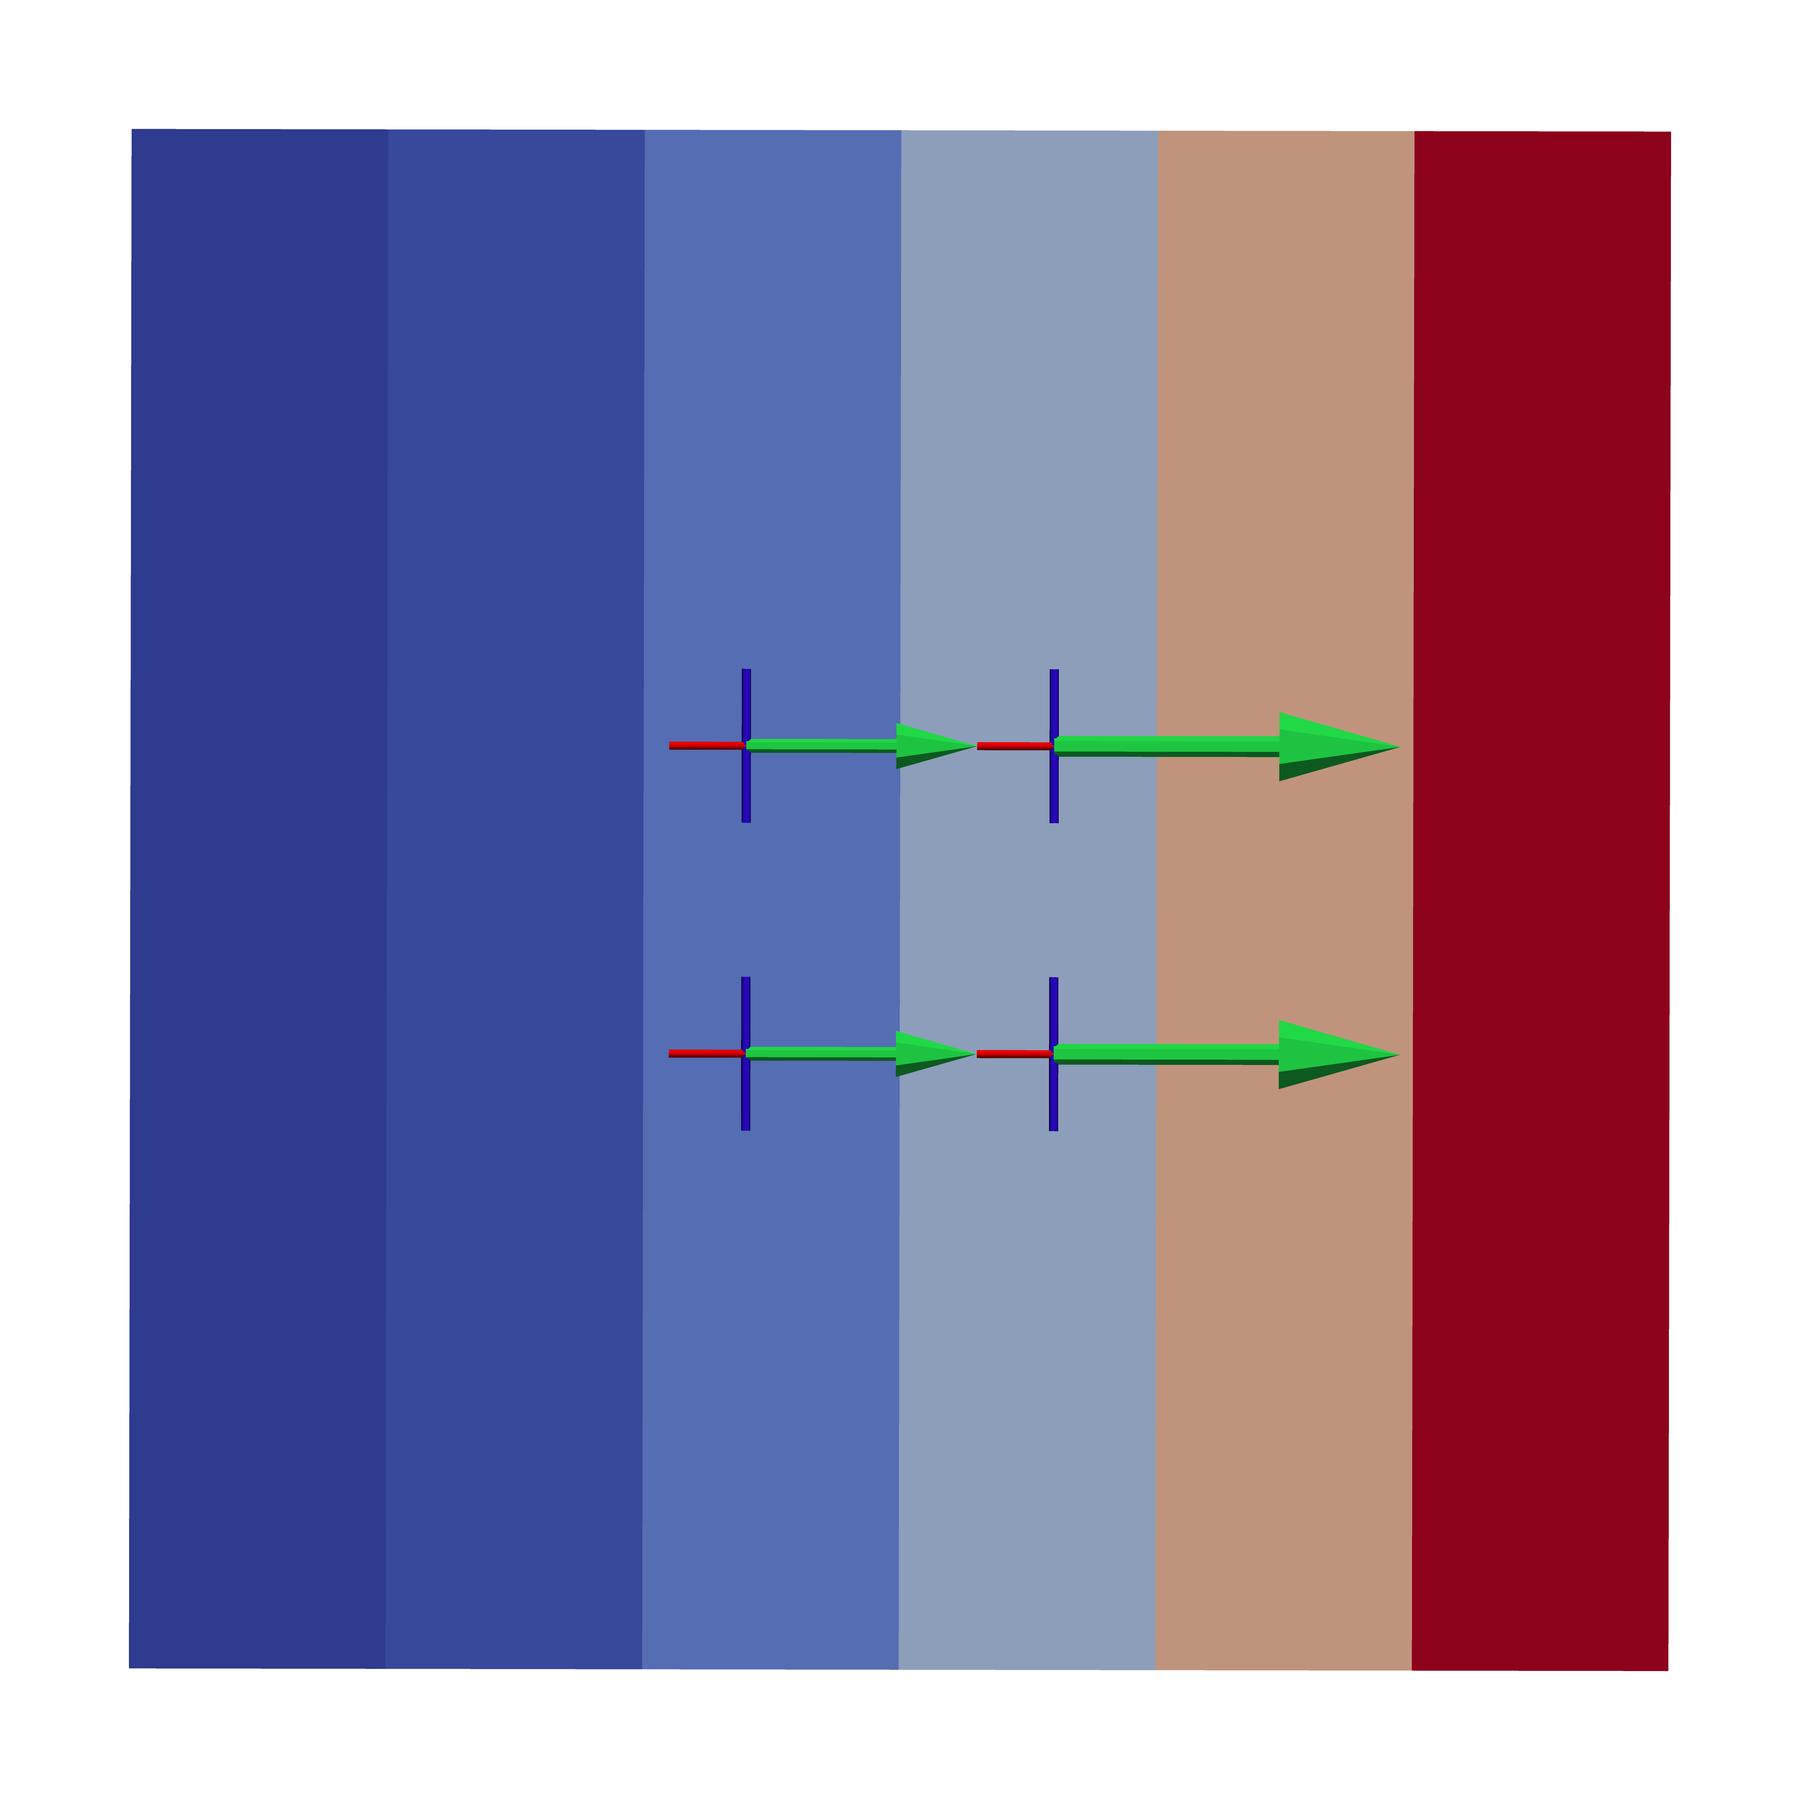
\includegraphics[width=\textwidth]{Images/gradient.png}
        \caption{Scalar field}
        \label{fig:gradient}
    \end{subfigure}
    \begin{subfigure}[b]{0.49\textwidth}
        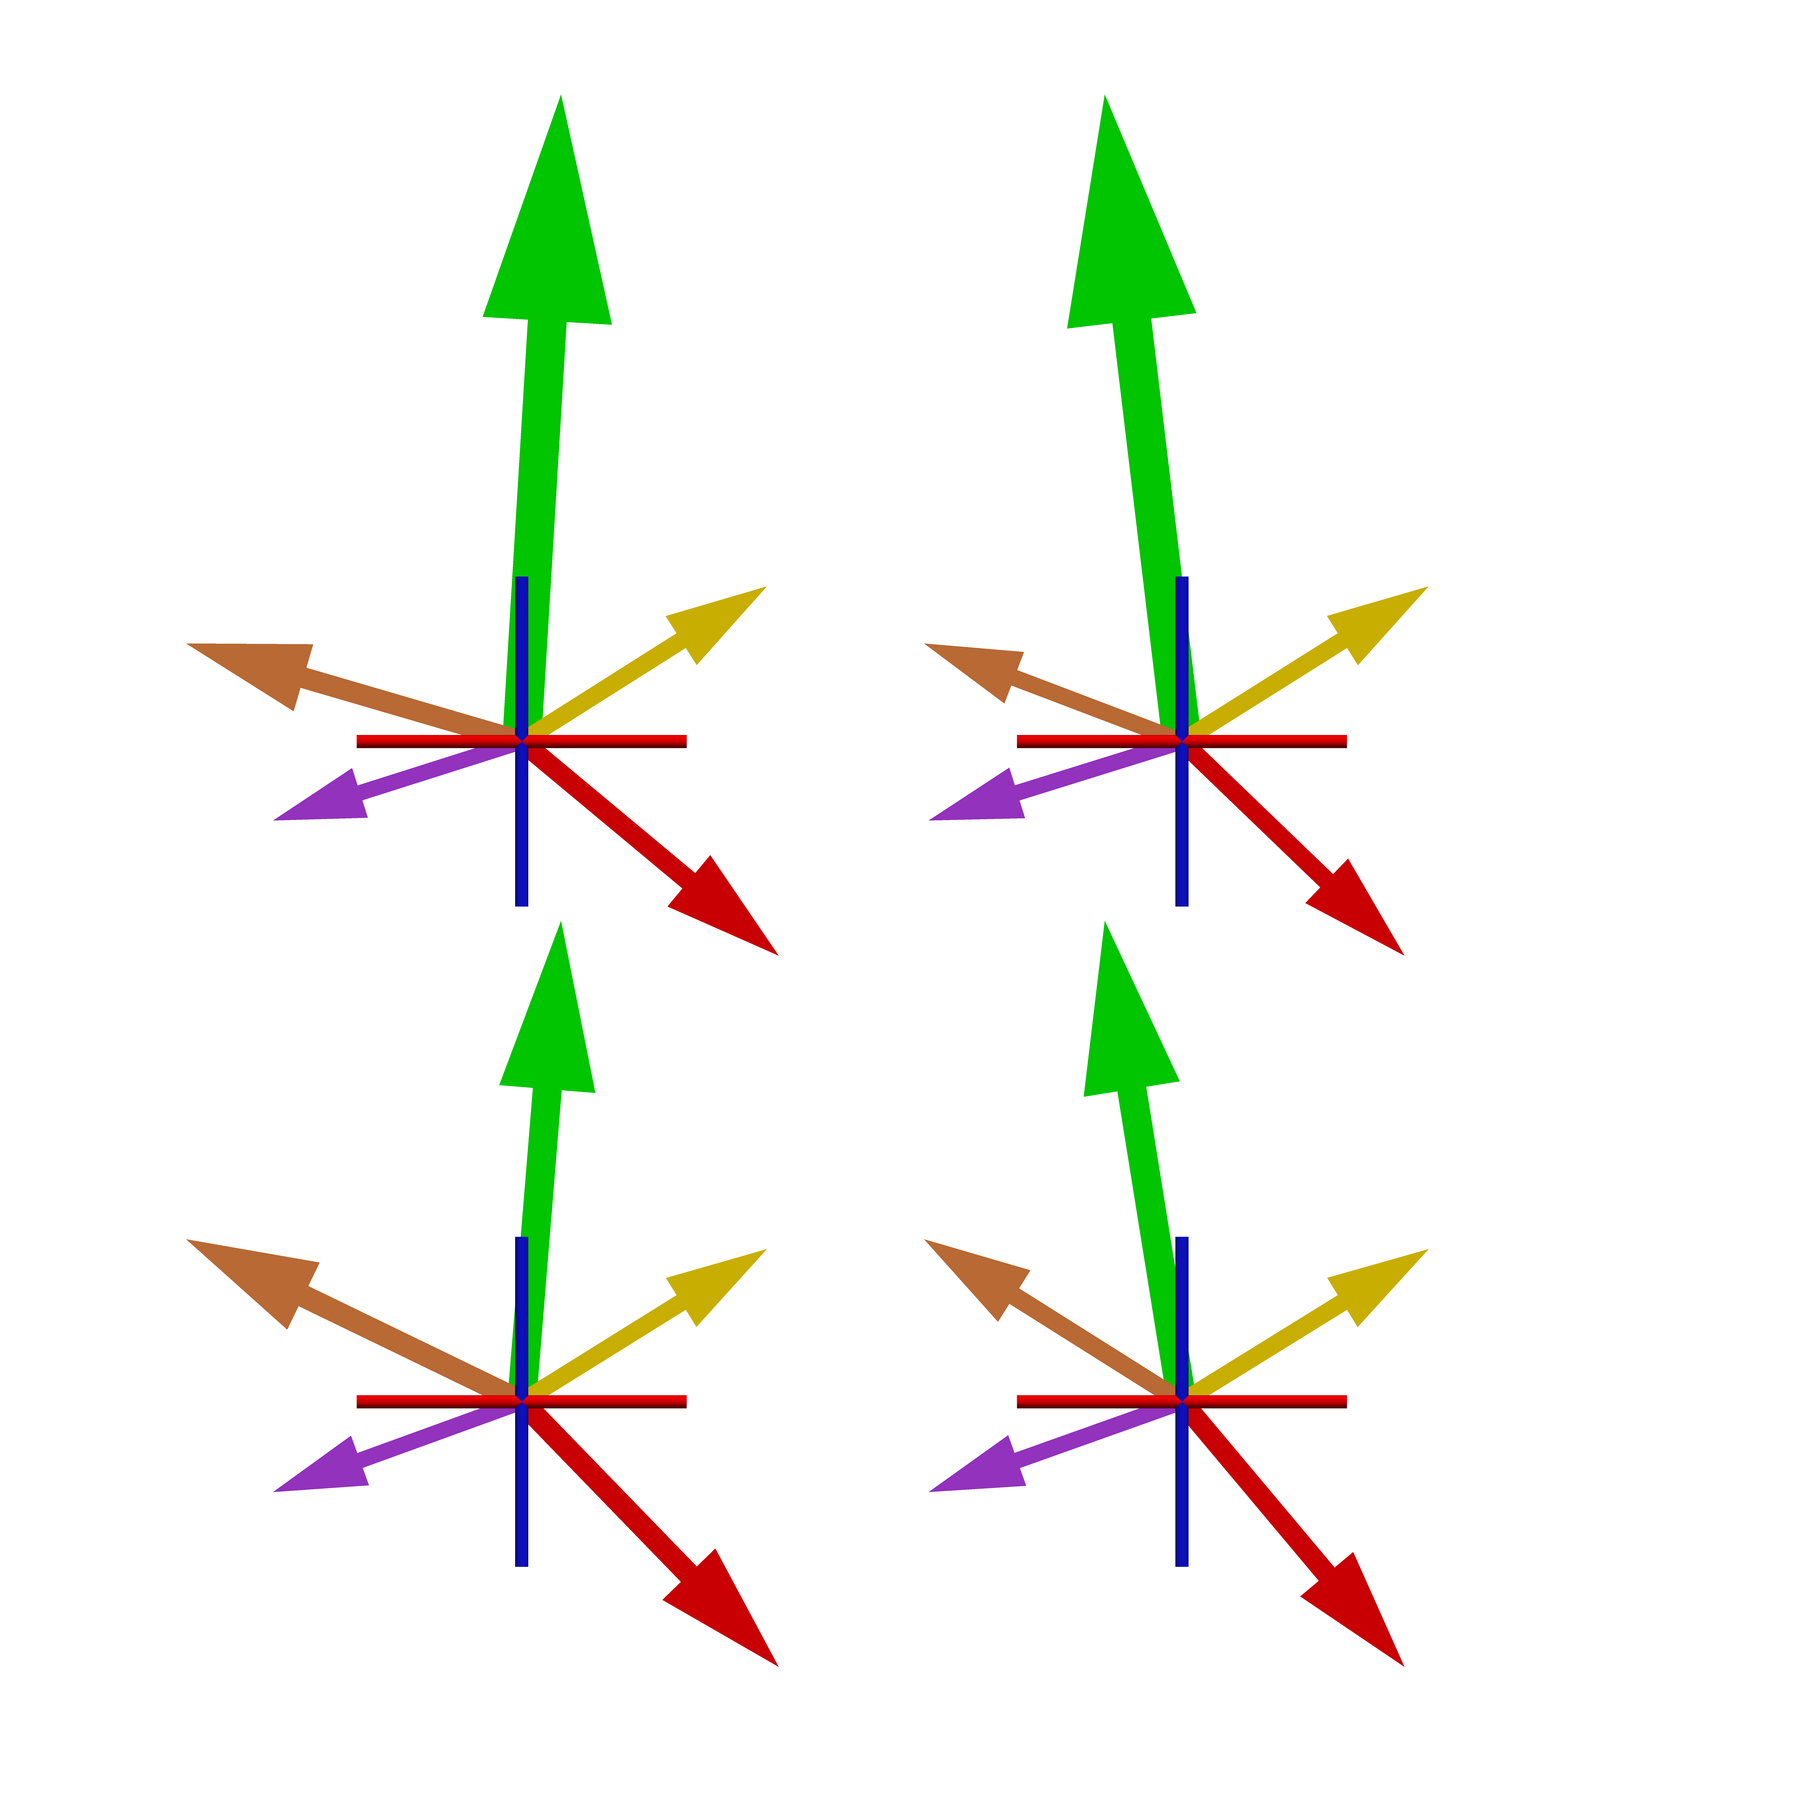
\includegraphics[width=\textwidth]{Images/samples.png}
        \caption{Samples}
        \label{fig:samples}
    \end{subfigure}
    \caption{\subref{fig:gradient} Gradients (green) in the field
    $f(x,y)=x^2$. The major eigenvector (red) is parallel to the
    gradient as the gradient only changes along the x-axis. The minor
    eigenvector (blue) is orthogonal to them with eigenvalue 0.
    \subref{fig:samples} Gradients (arrows) of samples from the Gaussian
    distribution over four rotated variants of the scalar field from
    \subref{fig:gradient} with their common eigenvectors. The
    eigenvectors (red and blue) are displayed as lines, as they yield no
    natural orientation and they coincide for every sample. These
    samples were obtained with the Eigendecomposition.}
    \label{fig:sampComp}
\end{figure}
\indent In this section we will cover the extraction of ridgesurfaces
from a 3-dimensional uncertain scalar field. The conservative approach
to extract the surface would be to calculate the dot product of the
gradient and the minor eigenvector at every node and apply the modified
Marching Cubes algorithm for isovalue 0. This faces us with a problem
that occurs when generating samples from a multivariate Gaussian
distribution. Depending on the uncertainty at the location, the
distribution of the values of the sample vector might vary heavily.
Figure~\ref{fig:sampComp} illustrates this problem with samples drawn
from a distribution in 2-dimensional space. Figure~\ref{fig:gradient}
shows the scalar field for the function $f(x,y) = x^2$ for $x, y \in
\{0,\dots,5\}$ and the gradients for the nodes of the cell in the
middle. As you can see, the gradients are parallel and aligned with
their major eigenvectors and their magnitude increases along $x$. We
rotated that field by 90 degrees three times, so that the gradient in
each field points orthogonal to the previous. Now we build the Gaussian
distribution for these fields and draw five samples using the
Eigendecomposition. We visualize the gradients of the sampled fields, as
they make the understanding of the samples easier.\\
\indent Figure~\ref{fig:samples} shows the gradients of each sample
together with their eigenvectors crossing at the respective nodes. The
individual samples relate to the parallel orientation of the original
fields, but their general direction is mixed up between the axes and
they vary in magnitude. The gradients of the green sample slightly point
towards each other, indicating that the field is increasing between the
nodes, which is never the case originally. Also interesting to note is
that the orientation of the eigenvectors is identical for every sample,
only the corresponding eigenvalue changes. Such heavy changes of the
direction of the gradient inbetween members are possible, as the
gradient always points towards the ridge. If the gradient is close to
it, small changes in the position of the ridge can result in big
directional changes. This makes the computation of ridge surfaces via
Marching Cubes quite inconsistent, even without noise on the data, as it
strongly relies on the orientation of the vectors to each other. If we
would now try to extract ridges with the conventional Marching Cubes
algorithm and only accept features where the dot product of the gradient
and the minor eigenvector is exactly zero, we would discard a lot of
valid ridge features. This is especially true for interpolated vectors
as a whole, due to numerical issues. We can try to challenge this
problem by giving a tolerance $t$ for the dot product to be zero, to
allow for detections where the gradient is close to being perpendicular
to the minor eigenvector, but the optimal value for the tolerance
depends on the uncertainty at the location and basically the knowledge
of where the ridge actually is.\\
\begin{figure}[t]
    \begin{subfigure}[b]{0.49\textwidth}
        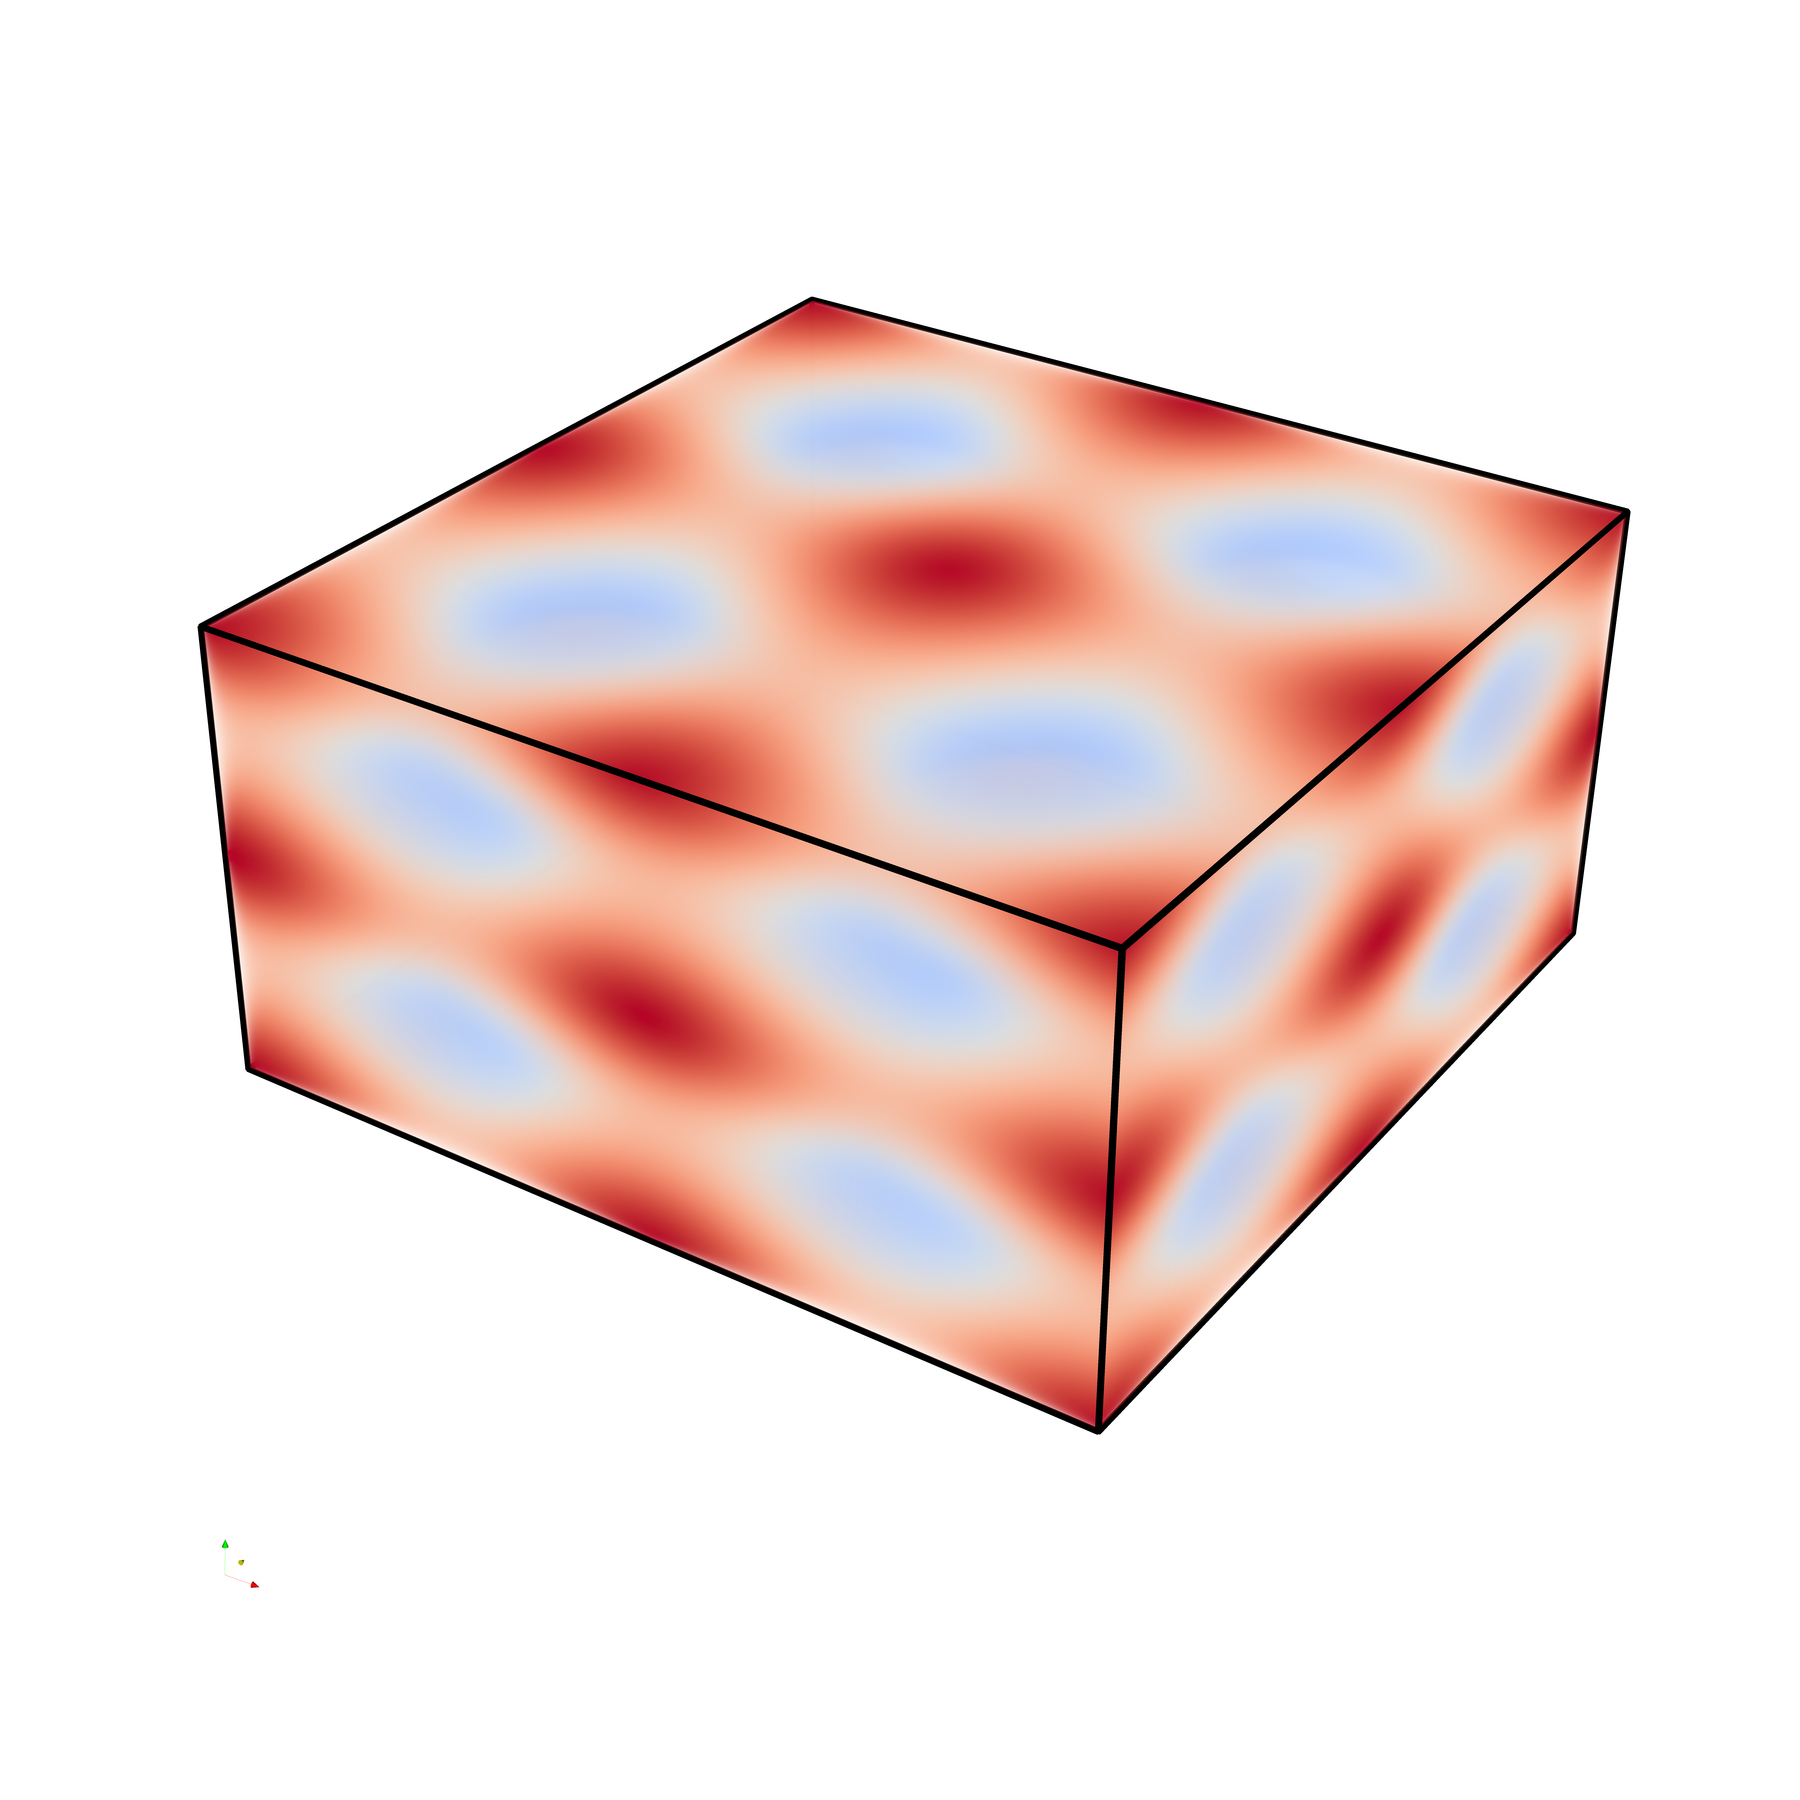
\includegraphics[trim=0 350 0 300, clip=true, width=\textwidth]{Images/sfield.png}
        \caption{Scalar field}
        \label{fig:sfield}
    \end{subfigure}
    \begin{subfigure}[b]{0.49\textwidth}
        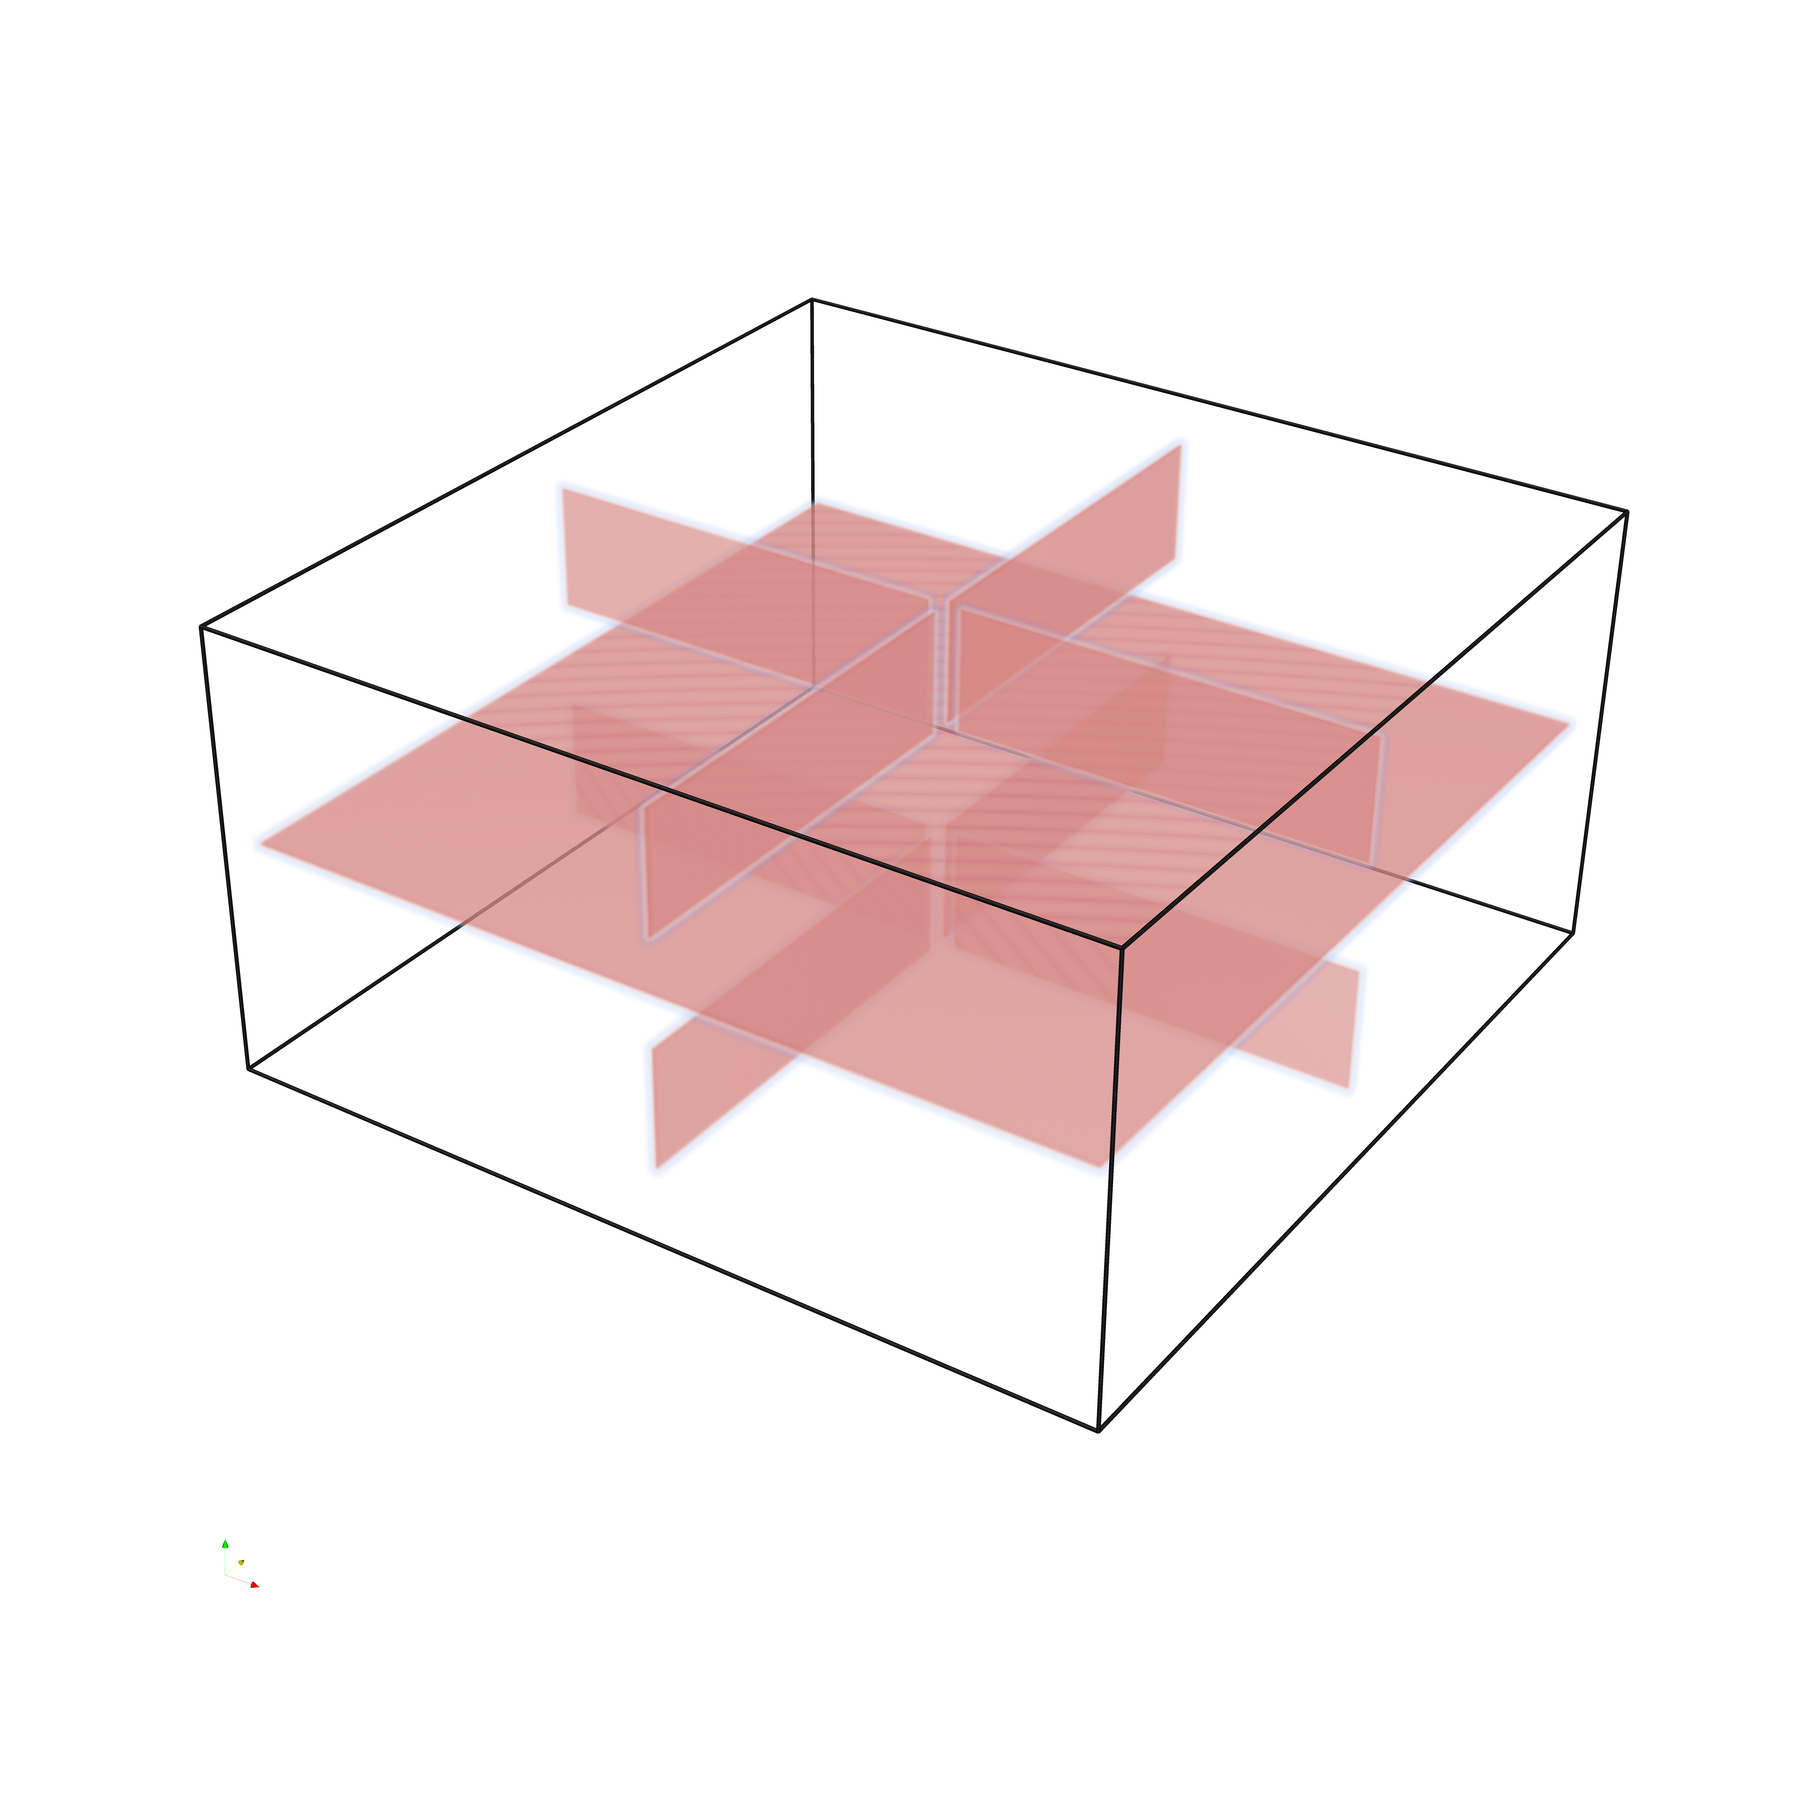
\includegraphics[trim=0 350 0 300, clip=true, width=\textwidth]{Images/ridge.png}
        \caption{Ridge surface}
        \label{fig:certainRidge}
    \end{subfigure}
    \caption{Ridge surface of the scalar field for the function
    $f(x,y,z)=\cos(x)+\cos(y) +\cos(z)$ with $x,y,z \in [0, 4\pi]$. The
    functions are periodic and therefore the ridges are symmetric. The
    z-axis is squished, even though it has the same data range as the
    other axes to ease the spatial understanding of the domain.}
    \label{fig:ridge}
\end{figure}
\indent To further illustrate this problem, we took the 3-dimensional
scalar field corresponding to the function $f(x,y,z) = \cos{(x)} +
\cos{(y)} + \cos{(z)}$ in the domain $[0, 4 \pi] \times [0, 4\pi] \times
[0, 4\pi]$. This function is periodical and therefore we can easily
shift the whole domain along a dimension by adding constants to $x, y$
or $z$. Figure~\ref{fig:ridge} shows the certain ridge surface for this
scalar field. As we have a cosinus function starting at 0 and ending at
$4\pi$ for every dimension, we have two full periods along either
dimension with their maxima in the middle at $2\pi$. This can easily be
seen in Figure~\ref{fig:certainRidge} with small surfaces orthogonal to
the $x$ and $y$ dimension and a bigger surface seperating the smaller
surfaces in $z$ direction. The ridge surfaces partly visible through the
bigger surface are identical to the ones above the big surface. To this
function, we add small positive and negative constants drawn from a
uniform distribution to $x, y$ and $z$, to generate an ensemble of
scalar fields, with their ridge moved around the original one. Now we
calculate the uncertain ridge surface of the distribution with 100
samples drawn per cell and only require the absolute of the dot product
to be smaller than $t=0.05$. The resulting surface is shown in
Figure~\ref{fig:MCridge}.
\begin{figure}
    \centering
    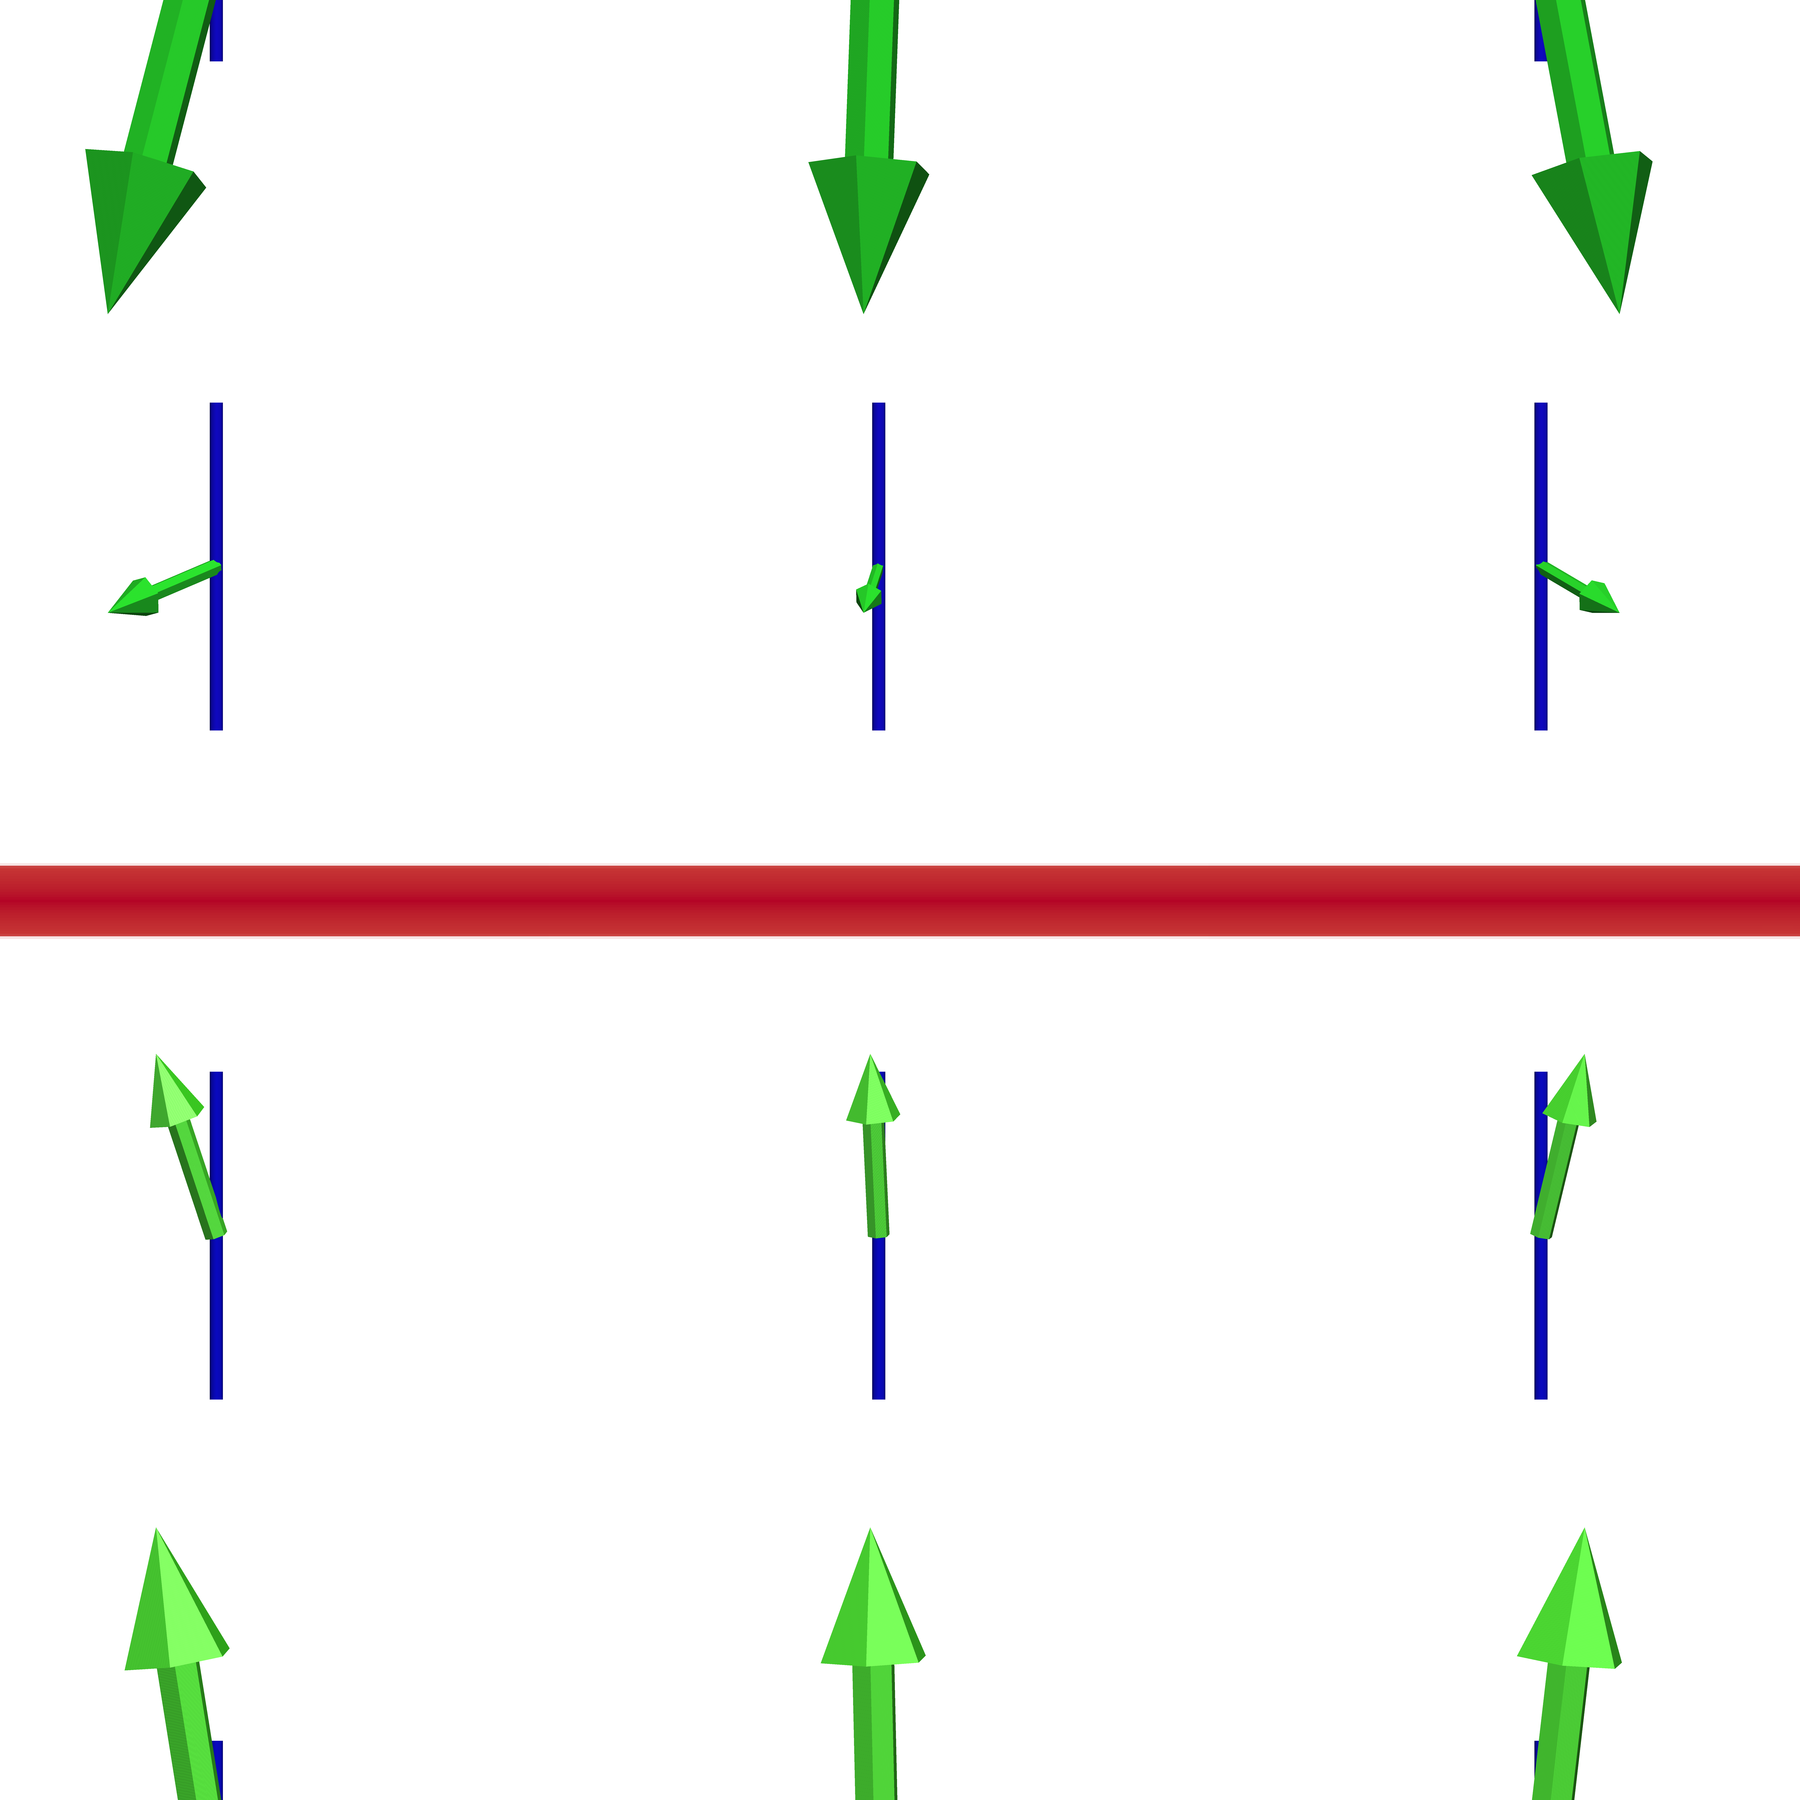
\includegraphics[trim= 0 300 0 305, clip=true, width=0.65\textwidth]{Images/weakridge.png}
    \caption{Gradients (green) and their minor eigenvectors (blue) close to
    a ridge at a volatile point. This is a sideview of a location where the
    holes from Figure~\ref{fig:MCridges} appear. Here, the gradient is almost
    parallel with its minor eigenvector until it is very close to the ridge.}
    \label{fig:volatile}
\end{figure}
Holes are visible at equidistant locations. They are at points, where
one cosinus function has a positive peak and the other two a negative
peak. Figure~\ref{fig:volatile} shows a sideview of such a location. The
gradient in the middle is almost parallel to its minor eigenvector, as
the other two cosinus functions have no change along their direction.
This makes the ridge feature volatile and the interpolation can be
problematic. These points are especially vunerable to small spatial
changes of the ridge, which causes them to drastically change
orientation when sampled. If we now increase the tolerance to try to
fill these holes, we pick up a lot of undesired features. For $t=0.25$
(Figure~\ref{fig:MCridgetol}) the holes are still visible, but already a
lot of false positives clutter the view. For $t=0.5$ (see
Figure~\ref{fig:MCridgetop}) the holes are barely visible in the broad
noise on the surface, but the smaller surfaces on top and bottom are
hard to distinguish from the surrounding false positives. This brings in
the need for an approximate ridge criterion that adapts to local
properties of the field, without being too restrictive or forgiving.

\begin{figure}[]
    \centering
    \begin{subfigure}[]{0.7\textwidth}
        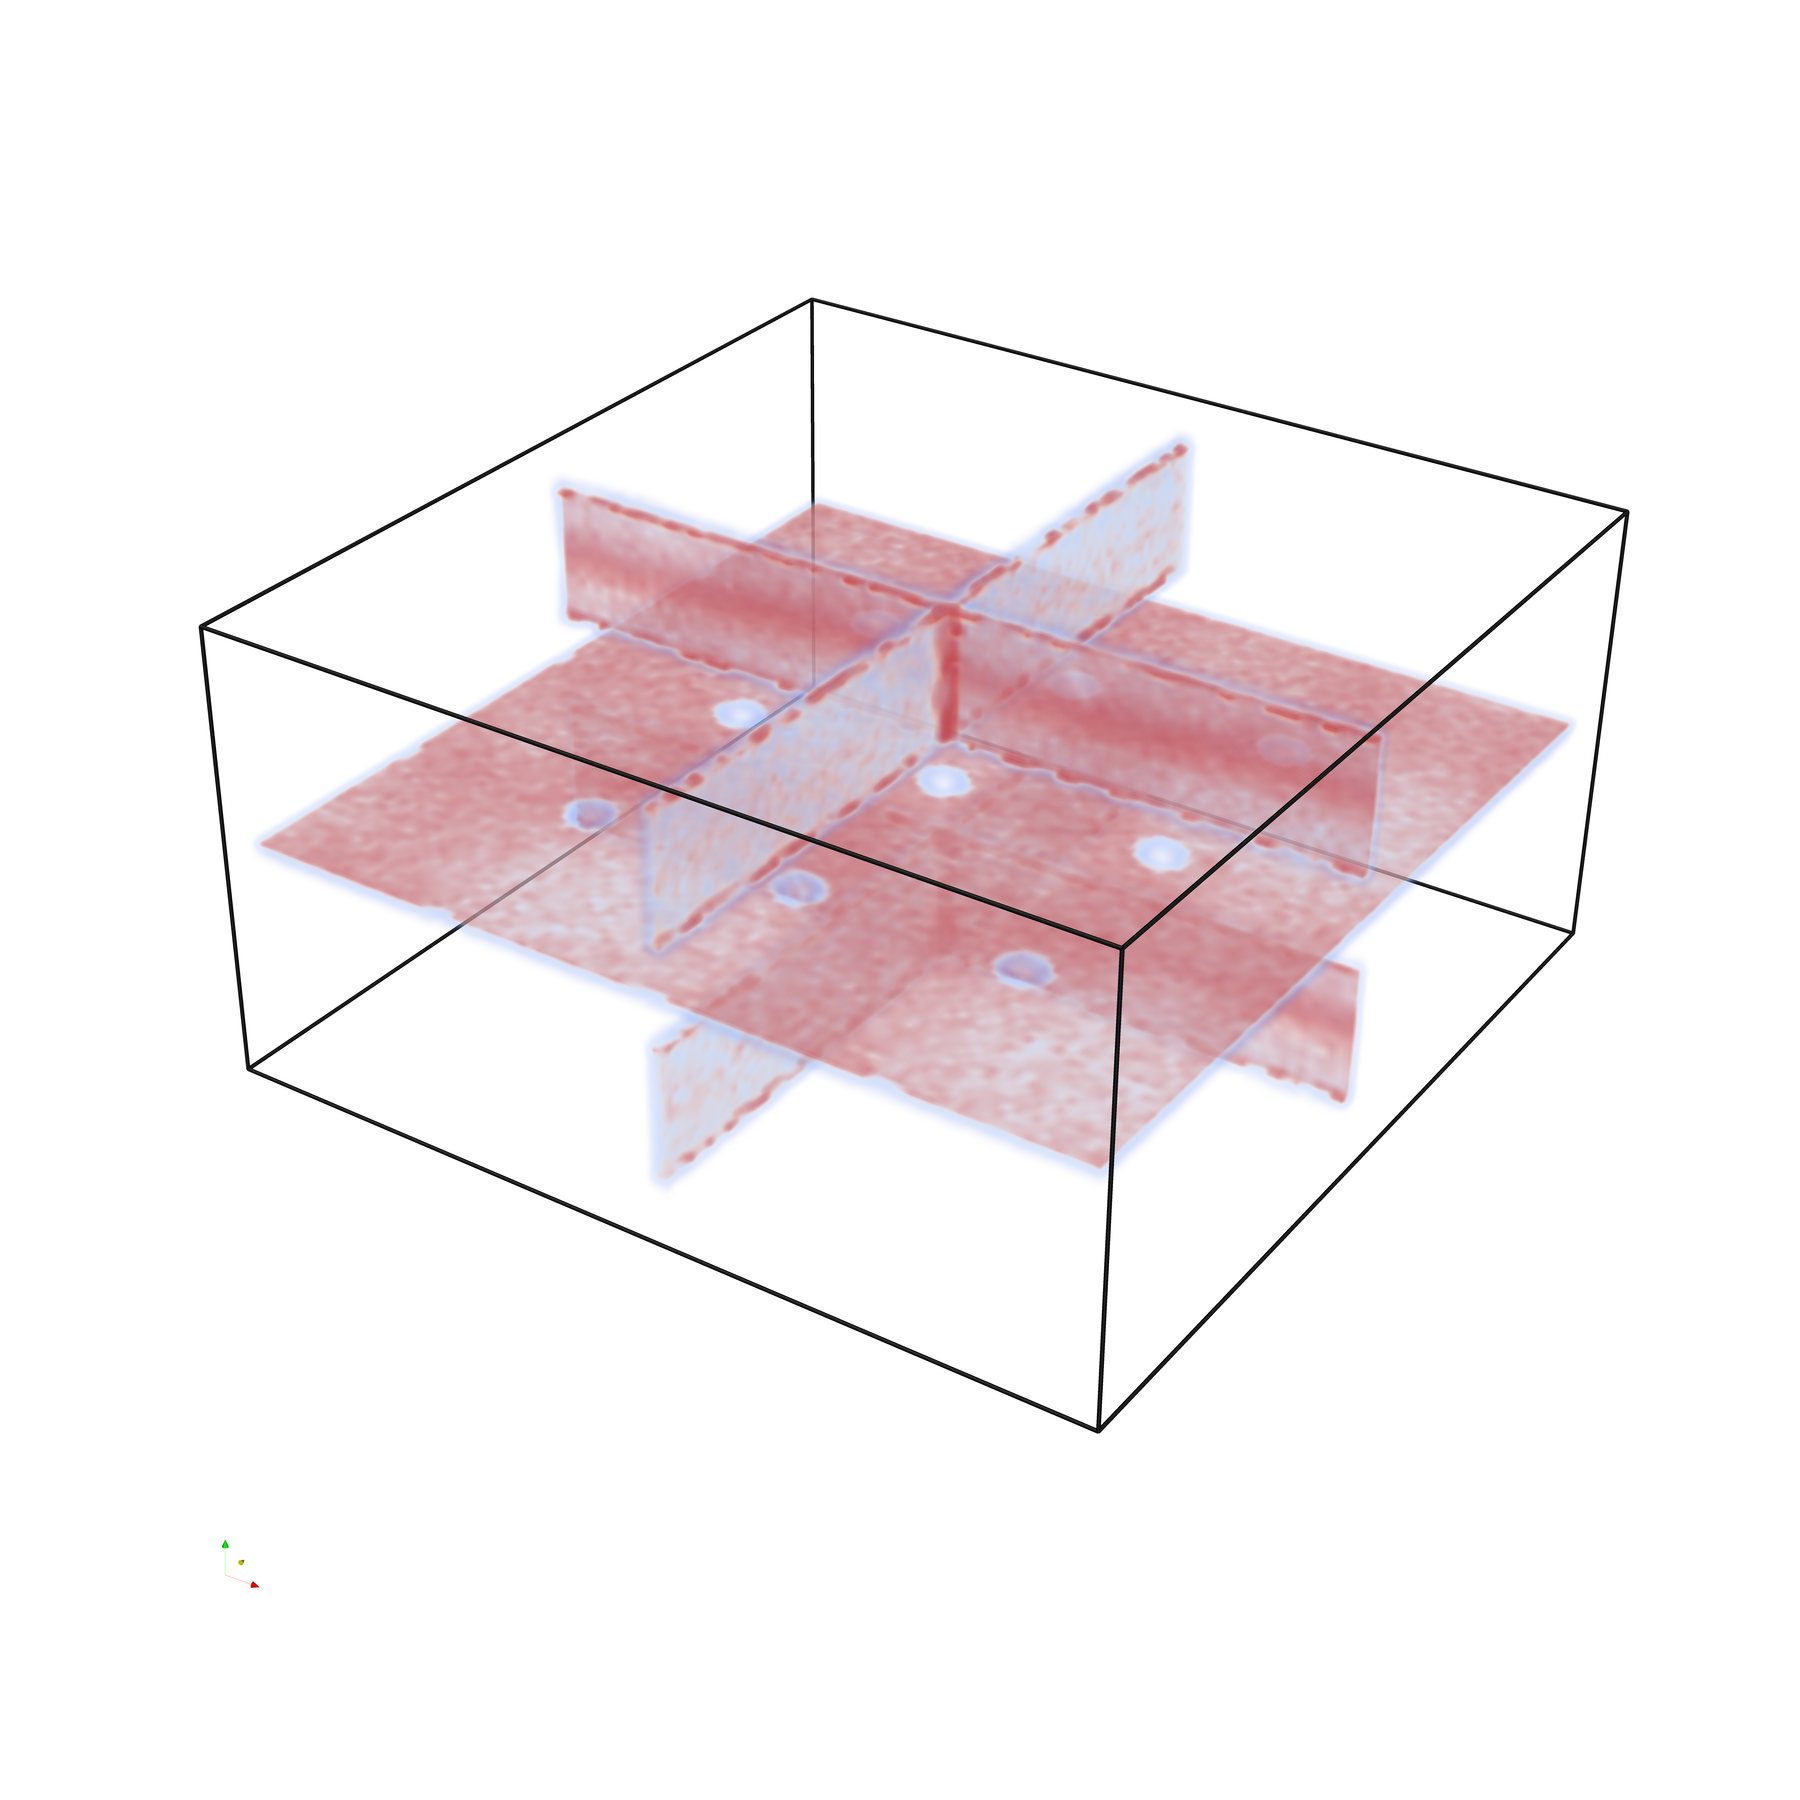
\includegraphics[trim=0 350 0 300, clip=true, width=\textwidth]{Images/MCridge.png}
        \caption{$t=0.05$}
        \label{fig:MCridge}
    \end{subfigure}
    \begin{subfigure}[]{0.49\textwidth}
        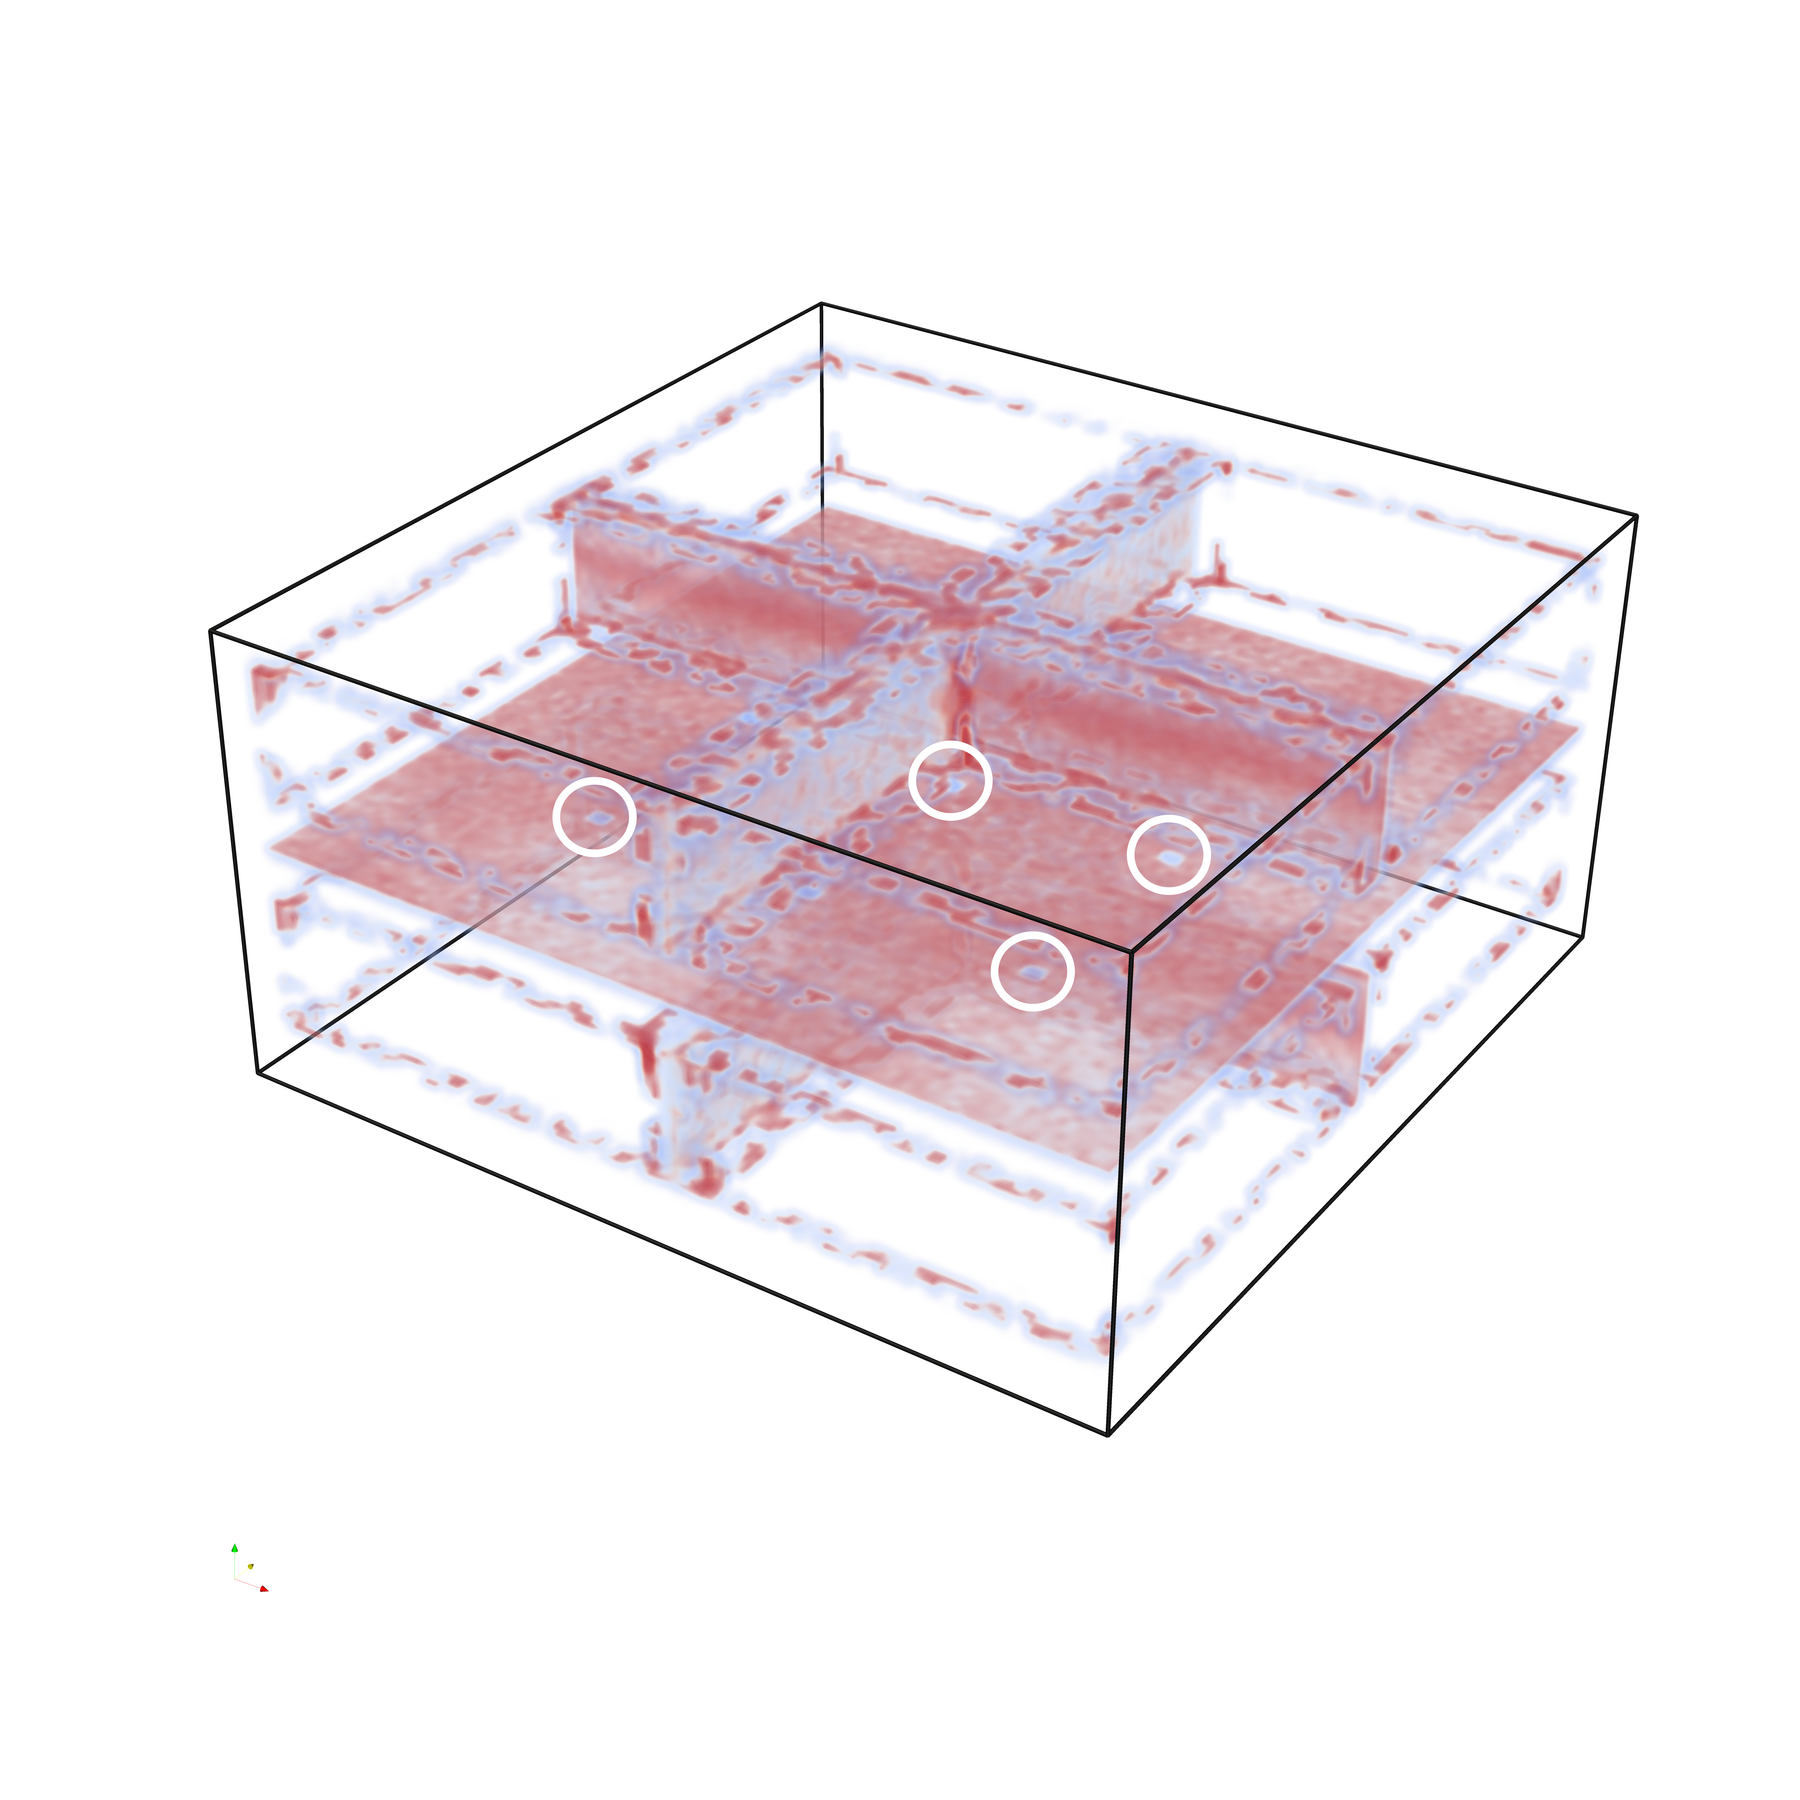
\includegraphics[trim=0 350 0 300, clip=true, width=\textwidth]{Images/MCridgetol.png}
        \caption{$t=0.25$}
        \label{fig:MCridgetol}
    \end{subfigure}
    \begin{subfigure}[]{0.49\textwidth}
        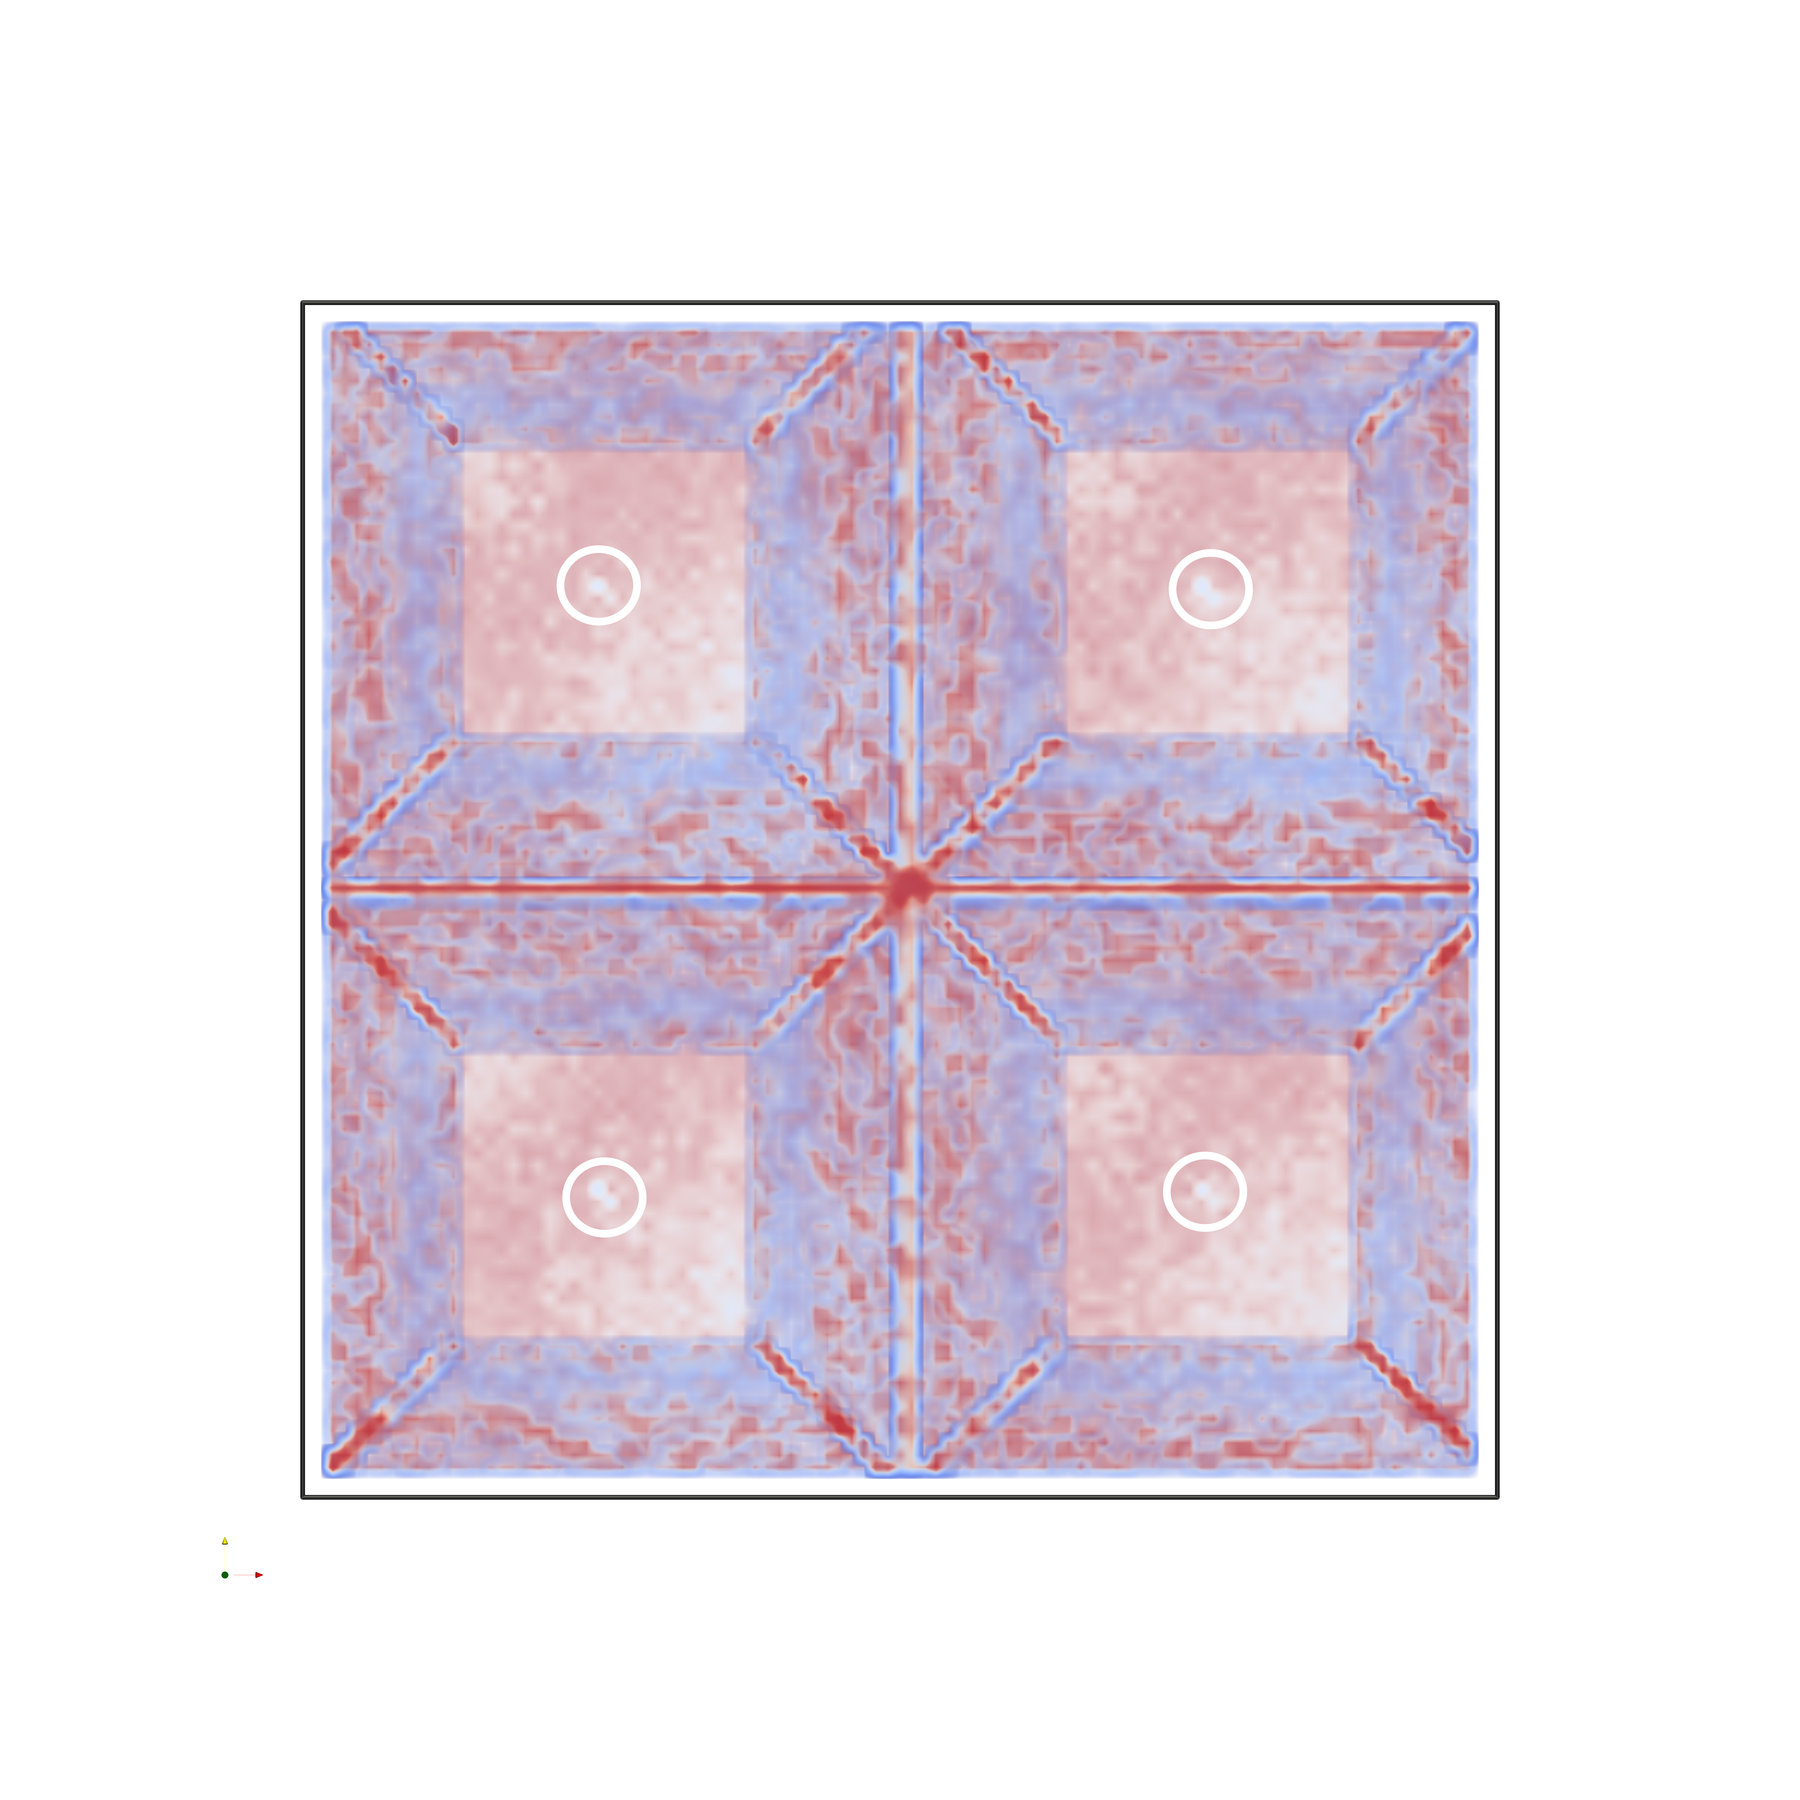
\includegraphics[trim=0 300 0 300, clip=true, width=\textwidth]{Images/MCridgetoltop.png}
        \caption{$t=0.5$}
        \label{fig:MCridgetop}
    \end{subfigure}
    \caption{Uncertain ridge surfaces from the Uncertain Marching Cubes
    algorithm for different tolerances for the dot product of the
    gradient and the minor eigenvector. For $t=0.05$ the big surface
    along $z$ has holes at the points where the ridge is weak and some
    undesired features at the edges of the upper and lower surfaces. As
    we increase the tolerance, the holes become smaller, but a lot more
    false positives occur. Figure~\subref{fig:MCridgetop} offers a top
    down view on the domain for $t=0.5$, as there is a lot of cluttering
    on the sides.}
    \label{fig:MCridges}
\end{figure}

%%%%%%%%%%%%%%%%%%%%%%%%%%%%%%%%%%%%%%%%%%%%%%%%%%%%%%%%%%%%%%%%%%%%%%%%
\subsubsection{Ridge Estimation}
%%%%%%%%%%%%%%%%%%%%%%%%%%%%%%%%%%%%%%%%%%%%%%%%%%%%%%%%%%%%%%%%%%%%%%%%

The underlying concept of the multivariate Gaussian sampling is to
approximate the distribution by drawing enough samples from it, so that
the variety of the set is covered well enough by the different samples.
This suggests that it might be a good idea to consider ridge criteria
that deliver an approximate result for the existence of a ridge in a
small area, without the need for strict parameters. For this, we can make
use of a basic principle. In a function $f(x)$, we can estimate the value
at $x + d$ with the derivative $f'(x)$, as it is the change of the
function along $x$. Multiplying $f'(x)$ with the distance gives us the
estimated change along $x$ and therefore
\begin{equation}
    f(x + d) \approx f(x) + d \cdot f'(x).
\end{equation}
The same is applicable for the gradient of a scalar field, where the
derivative is denoted by the Hessian matrix. The Hessian transforms the
gradient along its eigenvectors, scaled by the respective eigenvalues as
it is applied to the gradient. As mentioned in Section
\ref{sec:derivatives} the eigenvalues are the directional derivatives of
$\nabla S(x)$ and so the signs of the eigenvalues determine the direction
of the scaling. A positive eigenvalue scales along its eigenvector, as
the gradient increases in that direction. A negative eigenvalue scales
against the direction of the eigenvector, as the gradient decreases in
that direction. Remember Equation~\ref{eq:ridgeDot} stating that for
the existence of a ridge surface in three dimensions, the gradient has
to be orthogonal to the minor eigenvector $\epsilon_1$. Then the
gradient is aligned with the ridge feature and therefore the ridge is
orthogonal to $\epsilon_1$ as well. Following this, we know that
$\epsilon_1$ always points perpendicular to a potential ridge, and thus
the change of the gradient along $\epsilon_1$ gives us information about
its behaviour along the shortest direction to the ridge. The dot product
of the gradient with $\epsilon_1$ is equivalent to the change of the
gradient along $\epsilon_1$ and its extend into $\epsilon_1$. The
gradient always points into the direction of greatest ascend and
therefore, if we move along $\epsilon_1$, the components of the gradient
in $\epsilon_1$ direction will be scaled, reducing its extend into
$\epsilon_1$ direction just as much as it moves forward, provided that
the corresponding eigenvalue $\lambda_1$ is negative.
Figure~\ref{fig:criterion} visualizes this case for gradients close to a
ridge line. As the gradient will never point past the ridge, the dot
product becomes smaller moving along $\epsilon_1$. Now $\lambda_1$ gives
us an estimate of the change for a given distance $d$ along
$\epsilon_1$, as it is the directional derivative of the gradient.
Therefore we know, that if
\begin{figure}[]
    \centering
    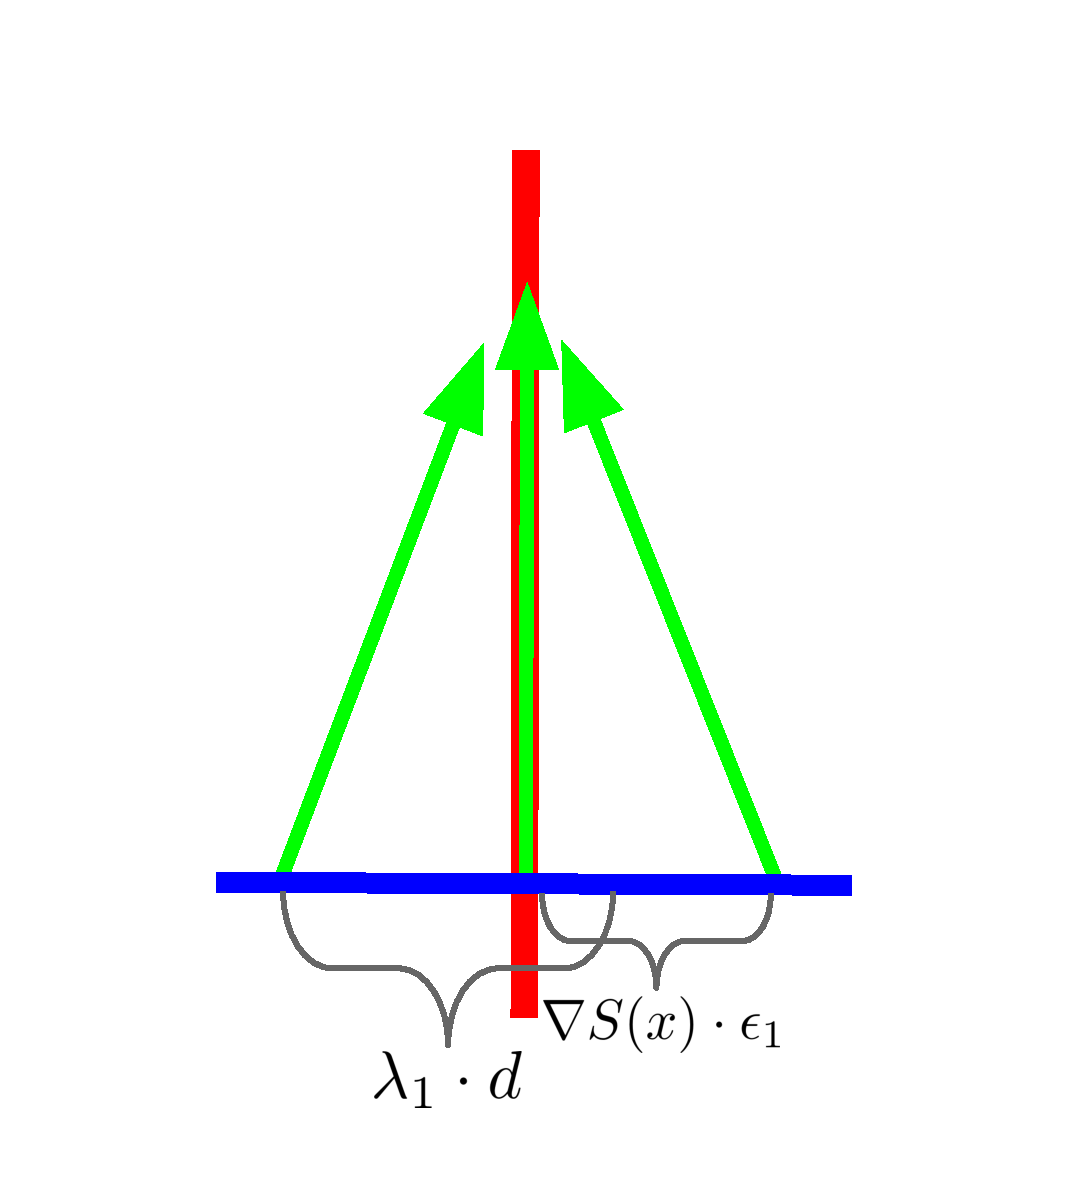
\includegraphics[trim=0 40 0 50, clip=true, width=0.4\textwidth]{Images/criterion.pdf}
    \caption{Illustration of gradients (green) close to a ridge line
    (red) in 2-dimensional space. The minor eigenvector $\epsilon_1$
    (blue) is orthogonal to the ridge. The gradients to the sides never
    point further than the ridge line, thus the dot product of the
    gradient and $\epsilon_1$ is at maximum the distance between the
    node and the ridge if the gradient is close. The dot product also
    denotes the change of the gradient into $\epsilon_1$ direction, as
    the gradient along $\epsilon_1$ will keep pointing towards the ridge
    and therefore become increasingly perpendicular to the eigenvector.
    Whereas the dot product only shows the change for its length, the
    eigenvalue shows the change for a uniform distance. Thus, if
    $\lambda_1$ multiplied with a scaling value is greater than the dot
    product $\nabla S(x) \cdot \epsilon_1$, the gradient flipped its
    direction and we therefore passed a ridge in the distance $d$.}
    \label{fig:criterion}
\end{figure}
\begin{equation}\label{eq:criterion}
    |\lambda_1 \cdot d| > |\nabla S(x) \cdot \epsilon_1|,\lambda_1 < 0
\end{equation}
is true, we passed a ridge somewhere in the distance $d$, as the
negative change of the gradient is greater than its extend into that
direction, implying that it flipped. Equation~\ref{eq:criterion} is our
new criterion for the existence of a ridge close to a node, which we
will call Ridge Estimation. This principle is applicable for all ridges
of co-dimension one. Back to our uncertain ridge surface extraction, a
suitable value for $d$ could now be the average distance of two nodes in
$x, y$ and $z$ dimension, as we are inspecting one cell at a time, but
in theory, $d$ can be adjusted to estimate over larger distances. We
apply Equation~\ref{eq:criterion} to every node of our sampled cell and
the probability for the existence of a ridge line inside this cell is
then the relative frequency of nodes for which the equation states true,
e.g., if it is true for 4 out of 8 nodes, the probability is $50\%$.
The probability for each sample is summed up and divided by the total
number of samples to get the final probability for the existence of a
ridge in that cell.\\
\indent Figure~\ref{fig:newmethod} shows the volume visualization for
the probabilities of the uncertain ridge calculation on the previous
data set using our new criterion. As you can see, the new method closed
all of the holes without adding undesired features to the result, but
the area of the ridge is now thicker. We have a smooth probability
distribution over the whole volume. The small surfaces on top and bottom
have slightly higher probabilities in the middle of their surfaces, as
the up and down movement of the individual members results in them
always having parts of their ridge at this location. A detailed analysis
of the difference of the methods is provided in Section
\ref{sec:evalExtr}.

\begin{figure}[]
    \centering
    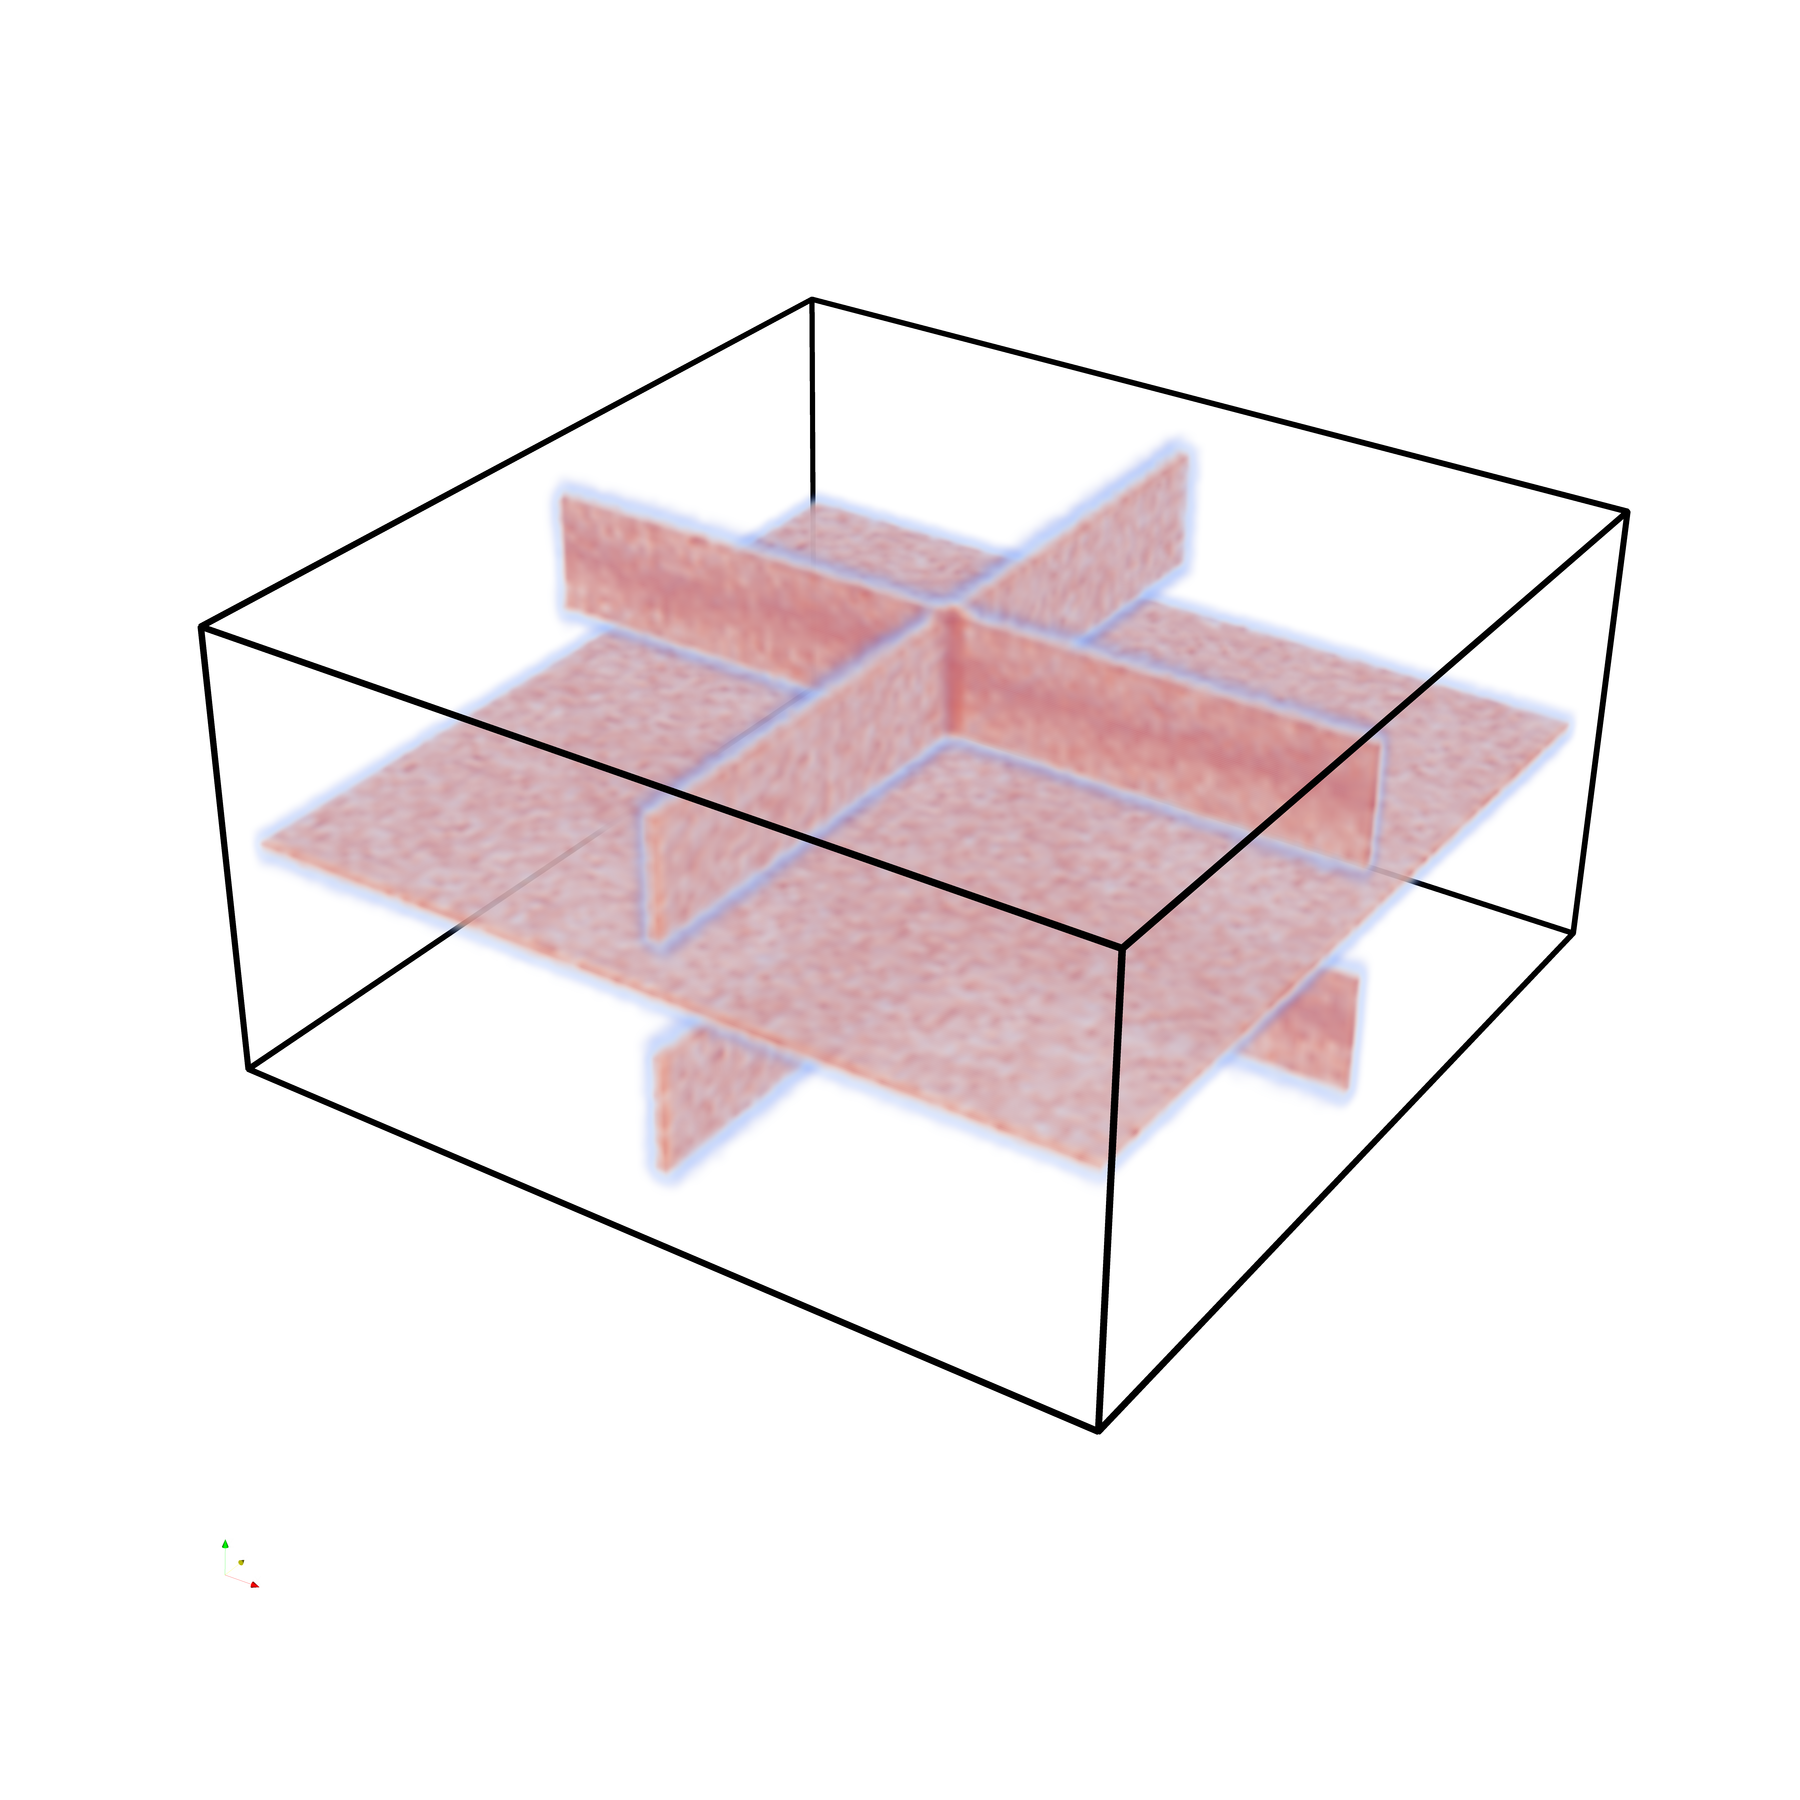
\includegraphics[trim=0 350 0 300, clip=true, width=0.7\textwidth]{Images/lowuncnew.png}
    \caption{Uncertain ridge surface for the set of shifted scalar
    fields from Figure~\ref{fig:MCridges}, calculated with the criterion
    from Equation~\ref{eq:criterion} and $d$ being the average spacing
    of the dimensions. The great surface perpendicular to $z$ has no
    holes and we are free from undesired features. The choice of $d$
    determines the thickness of the ridge. The samples were drawn using
    the Eigendecomposition.}
    \label{fig:newmethod}
\end{figure}

%%%%%%%%%%%%%%%%%%%%%%%%%%%%%%%%%%%%%%%%%%%%%%%%%%%%%%%%%%%%%%%%%%%%%%%%
\subsubsection{Filtering}
%%%%%%%%%%%%%%%%%%%%%%%%%%%%%%%%%%%%%%%%%%%%%%%%%%%%%%%%%%%%%%%%%%%%%%%%

Even though our new criterion delivers an estimate of the existence of a
ridge in the range of $d$ around a node without sampling a lot of false
positives, we might still want to filter by other criteria measurable in
a local cell. The magnitude of the eigenvalues is an indicator for the
sharpness of a ridge. This comes from their property of being the
directional derivative. A high absolute value for $\lambda_1$ means that
there is a big directional change along $\epsilon_1$. Therefore, if we
demand for a higher negative value of $\lambda_1$ at the node, we can
filter flatter ridge features without the need for interpolating the
Hessian at the ridge. Furthermore we can filter cells where the ordering
of the eigenvectors is inconsistent by the shape of their principal
component subdomain. False ordering is due to inflection points, where
the values of the field are close to zero and therefore there is very
few change in either direction, causing the eigenvalues to be very
similar. Therefore the ordering by Eberly can result in eigenvectors
changing their orientation drastically between nodes. The subdomain
denoted by the ellipsoid around the set of eigenvectors then is more
planar than linear. This can be observed by the relation of the second
largest eigenvalue to the largest eigenvalue. The PCA filter therefore
discards cells where the second largest eigenvalue is greater than a
given percentage of the largest eigenvalue of the PCA subdomain. Both
these filters are also applicable for the conservative ridge extraction
with Uncertain Marching Cubes and the Parallel Vectors Operator, with
the eigenvalues and vectors at the interpolated point between the nodes.
With our methods explained in detail, we can now start to evaluate the
results obtained from different data sets.